\documentclass[12pt]{article}
\usepackage[utf8]{inputenc}
\usepackage[ngerman]{babel}
\usepackage[T1]{fontenc}
\usepackage{cite}
\usepackage{float}
\usepackage{todonotes}

%Listings
\usepackage{listings}
\lstset{
    basicstyle=\ttfamily,
    columns=fullflexible,
    frame=single,
    breaklines=true,
    postbreak=\mbox{\textcolor{red}{$\hookrightarrow$}\space},
}

%Bilder importieren
\usepackage{graphicx}
\graphicspath{ {./img/} }

%Referenzen
\usepackage{hyperref}
\hypersetup{
    colorlinks,
    citecolor=black,
    filecolor=black,
    linkcolor=black,
    urlcolor=black
}

%Variable Textbausteine
\newcommand{\ipName}{Herr Maier }
\newcommand{\thesisTitle}{Menschzentrierte Gestaltung einer Terminvereinbarungssoftware}

%Metadaten
\title{\thesisTitle}
\author{Johannes Schnirring}

%Hier beginnt der Inhalt
\begin{document}

%Titelseite
\begin{titlepage}
    \centering
    {\scshape\Huge \thesisTitle \par}
    \vspace{1cm}
    {\scshape\Large \textbf{Bachelorarbeit}\par}
    \vspace{1.5cm}
    \begin{tabular}{r l}
        {\Large Studierender:}   & {\Large Johannes Schnirring}                     \\ \\
        {\Large Matrikelnummer:} & {\Large 33422833}                                \\ \\
        {\Large Studiengang:}    & {\Large Informatik (PO 2018) }                   \\ \\ \\ \\
        {\Large Erstprüferin:}   & {\Large Prof. Dr. Claude Draude }                \\
                                 & {\Large Gender/Diversity in Informatiksystemen } \\ \\
        {\Large Zweitprüfer:}    & {\Large Prof. Dr. Albert Zündorf }               \\
                                 & {\Large Software Engineering }                   \\ \\ \\ \\
        {\Large Semester:}       & {\Large Wintersemester 2022}                     \\ \\
        {\Large Datum:}          & {\Large \today}                                  \\ \\
    \end{tabular}
    \vfill
    {\large Universität Kassel}
\end{titlepage}

%Eidesstattliche Erklärung
\thispagestyle{empty}
\begin{center}
    \Large\scshape Eidesstattliche Erklärung
\end{center}
Ich erkläre an Eides statt, dass ich die vorliegende Arbeit selbständig
verfasst, andere als die angegebenen Quellen/Hilfsmittel nicht benutzt, und die
den benutzten Quellen wörtlich und inhaltlich entnommenen Stellen als solche
kenntlich gemacht habe.
\vspace*{5cm}
\noindent
\begin{minipage}[h]{0.4\linewidth}
    Kassel, am\dotfill\\
    \vspace*{2.5mm}
\end{minipage}
\hspace*{0.1\linewidth}
\begin{minipage}[h]{0.5\linewidth}
    \begin{center}
        \dotfill\\
        (Unterschrift)
    \end{center}
\end{minipage}
\newpage

%Inhaltsverzeichnis
\tableofcontents
\newpage

%Einbinden der eigentlichen Kapitel
\chapter{Einleitung}

\section{Zusammenfassung}

Diese Arbeit beschäftigt sich mit dem Entwicklungsprozess einer Software zur
Terminvergabe von Beratungsterminen der Studienberatung der Universität Kassel.
Der Entwicklungsprozess wird mit Methoden des \textbf{Human Centered Design}
begleitet und umgesetzt. Diese Arbeit erklärt die verwendet Methoden, sowie die
dahinterliegende Theorie. Die Software zur Terminvereinbarung wird
implementiert, wobei alle Schritte des Entstehungsprozesses beschrieben,
dokumentiert und ausgewertet werden.

Die allgemeine Studienberatung der Universität Kassel setzt die Software
Stubegru bereits seit 6 Jahren zum Management ihrer Beratungstermine,
Abwesenheiten und als Wissensdatenbank ein. Das Modul zur Vergabe der
Beratungstermine soll nun grundlegend neu implementiert werden und noch besser
an die Bedürfnisse der Mitarbeitenden angepasst werden. In Zusammenarbeit mit
\ipName, als Ansprechpartner aus der Abteilung Studium und Lehre, wird dieses
neue Modul entwickelt, designt und implementiert.\\ Die Bachelorarbeit
begleitet diesen praktischen Prozess, indem theoretische Grundlagen erläutert
werden und alle Entwicklungsschritte beschrieben werden. Die Theorie des Human
Centered Design gibt vor, wie ein Gestaltungsprozess von Software aussehen
kann. Neben grundlegenden Herangehensweisen bringt diese Theorie einige
Methoden mit, die im Laufe des Entwicklungsprozesses angewandt werden. Hierzu
gehört beispielsweise das \textbf{Interview im Kontext}, das in dieser Arbeit
erklärt wird und dessen praktische Umsetzung dokumentiert, ausgewertet und
kritisch hinterfragt wird.

\section{Motivation}

\subsubsection{Historische Entwicklung}
Wir leben in einem Zeitalter, in dem immer mehr Prozesse des täglichen Lebens
durch technische Systeme wie Software begleitet werden. In dieser Situation ist
es von hoher Relevanz, dass alle Menschen unserer Gesellschaft die Möglichkeit
haben, diese Systeme gleichermaßen zu nutzen und zu verstehen. In den Anfängen
der Softwareentwicklung wurde Software in der Regel aus Sicht der
verarbeitenden Maschine gedacht: Wie kann die Maschine die gegebenen Aufgaben
möglichst schnell, fehlerfrei und Effizient abarbeiten? Die Nutzenden dieser
Maschinen war meist ein eingeschränkter, speziell dafür ausgebildeter
Personenkreis. Diese Situation hat sich gänzlich verändert. Fast jeder Mensch
agiert heute viele Male am Tag mit technischen, softwaregetriebenen Systemen,
wei zum Beispiel Bankautomaten, Smartphones, Supermarktkassen oder Computern.
Außerdem wird der Umgang mit solchen Systemen durch neue Entwicklungen wie
Sprachsteuerung oder Touchscreens immer interaktiver und unmittelbarer. Somit
ist es enorm wichtig, dass alle diese Systeme eine klare und
nutzungsfreundliche Schnittstelle für die bedienenden Personen bieten.

\subsubsection{Rolle des Human Centered Design}
Der Ansatz des \textbf{Human Centered Design} setzt an genau dieser Stelle an,
indem er Grundkonzepte und Methoden vermittelt, die das Design von
Benutzerschnittstellen thematisieren. Das Kernkonzept des Human Centered Design
ist es den Blickwinkel aus der Perspektive der Nutzenden zu wählen. Die zu
entwickelnden Systeme sollen Schnittstellen anbieten, die intuitiv und einfach
zu verstehen sind. Prozessabläufe sollen aus Sicht des Nutzenden abgebildet
werden und möglichst wenig durch technische Hintergründe eingeschränkt sein.

\subsubsection{Praktische Anwendung Stubegru}
Dieser Designansatz soll in dieser Bachelorarbeit genauer untersucht werden.
Zum einen, indem die theoretischen Hintergründe genauer erläutert und Methoden
präzise erklärt werden. Den wesentlichen Teil dieser Arbeit stellt aber die
Dokumentation der praktischen Anwendung all dieser Methoden und Konzepte dar.
Dies soll am Beispiel einer Software zur Terminvergabe in der Studienberatung
an der Universität Kassel durchgeführt werden. Das entsprechende Modul für
diese Software soll im Rahmen dieser Arbeit geplant, gestaltet, implementiert
und getestet werden. All diese Schritte werden schriftlich aufgearbeitet,
festgehalten und hinterfragt. Das Ziel dieser Arbeit soll es also sein, den
Designzyklus des Human Centered Design am praktischen Beispiel einer
Terminvergabe-Software anzuwenden. Die bestehenden wissenschaftlichen
Erkenntnisse im Bereich der menschzentrierten Gestaltung sollen somit
erarbeitet, vertieft und auf Praxistauglichkeit geprüft werden. Ein weiterer
wichtiger Bestandteil ist schließlich die theoretischen und methodischen
Grundlagen im Hinblick auf die gewonnenen praktischen Erfahrungen zu
hinterfragen und deren Praxistauglichkeit zu diskutieren.

\section{Aufbau}
Zu Beginn der Arbeit werden zunächst die verwendeten Grundlagen und Methoden
des Human Centered Design genauer erläutert und klar definiert. Exemplarisch
für eine Methode wird das Konzept des Interviews im Kontext genauer betrachtet
und eingeführt. Das nächste Kapitel beschäftigt sich mit der praktischen
Durchführung der Entwicklung des Softwaremoduls zur Terminvereinbarung anhand
der vorher vorgestellten Methoden. Um dem Lesenden einen Eindruck über den
aktuellen Einsatz der betrachteten Software an der Universität zu geben, wird
zunächst der Kontext im Team der entsprechenden Abteilung erläutert.
Anschließend wird die eingesetzte Software genauer vorgestellt und deren
Entwicklungsgeschichte aufgegriffen. Im weiteren Verlauf soll thematisiert
werden, aus welchen Gründen eine Überarbeitung dieser Software notwendig ist
und welches Ziel die allgemeine Studienberatung damit beabsichtigt. Im nächsten
Schritt wird ein Interview im Kontext mit einem Mitarbeitenden der
Studienberatung durchgeführt, dokumentiert und ausgewertet. Die aus den
Wünschen und Bedürfnissen der Nutzenden entstehenden Anforderungen sollen
ebenfalls zusammengefasst und dargestellt werden. Als nächster Schritt soll die
praktische Umsetzung der technischen Anforderungen an die Software skizziert
werden. Implementierungsdetails, Screenshots und Codeschnipsel sollen in diesem
Teil die Dokumentation der Umsetzung veranschaulichen. Als letzter Aspekt
dieses Kapitels soll das Feedback der Nutzenden bei Vorstellungen von
Prototypen und ersten Ergebnissen festgehalten und aufbereitet werden. Im
letzten Kapitel wird schließlich das Ergebnis des durchgeführten
Entwicklungsprozesses dargestellt. Die eingesetzten Methoden werden nochmals
aufgegriffen und kritisch hinterfragt: An welchen Stellen können die
theoretischen Grundlagen des Human Centered Design den Entwicklungsprozess in
der Praxis tatsächlich sinnvoll unterstützen? Gab es eventuell auch Methoden,
die in der praktischen Umsetzung problematisch waren oder noch optimiert werden
könnten? Der letzte Teil dieser Arbeit gewährt schlussendlich einen Ausblick
auf weitere Einsatzmöglichkeiten des Human Centered Design und die weitere
Entwicklung der Software in der Studienberatung der Universität Kassel.



% Hier wird die Problemstellung im Kontext
% einer Anwendung dargestellt und der Inhalt der Arbeit kurz vorweggenommen. Welches Problem wurde
% gelöst, warum ist das relevant? Wie ist die Vorgehensweise? Was wurde thematisch eingegrenzt, was
% wurde ausgegrenzt? Wichtig ist es, den eigenen Beitrag in wenigen prägnanten Sätzen herauszuarbeiten. (Das Fazit soll sich zum Schluss auf diese Beiträge beziehen, um der Arbeit eine erzählerische
% Klammer zu geben.) Die Einleitung endet mit einem Überblick über die Arbeit – hierbei werden die
% Inhalte der einzelnen Kapitel knapp umschrieben

\chapter{Methoden}
\label{chapter:methods}

\section{Human Centered Design}
Human Centered Design ist eine Methode die den Entwicklungsprozess von
interaktiven Systemen und Software beschreibt. Die Kernthese des Human Centered
Design ist, dass die Nutzenden der Systeme im Mittelpunkt aller Entwicklungs-
und Designprozesse stehen.

Die Entwicklung von Software war in den Anfängen geprägt von den technisch sehr
eingeschränkte Möglichkeiten des Computers. Software wurde also größtenteils so
entwickelt, dass sie möglichst problemlos und effizient auf dem entsprechenden
Computer ausgeführt werden kann. Alle Entwicklungsprozesse wurden also aus
Perspektive der ausführenden Maschine gedacht. Der Ansatz des Human Centered
Design setzt dieser maschinenzentrierten Vorgehensweise eine klare Alternative
entgegen. Martin Ludwig Hofmann beschreibt den Grundgedanken in \glqq{} Human
Centered Design\grqq{} so: \glqq{} [Es geht] nicht darum, mit Geräten zu
denken, sondern mit Menschen und ihren Weltanschauungen\grqq{}. \cite{hcd} Wie
im Kapitel Motivation ausführlich erläutert gewinnt dieser Ansatz in der
heutigen Zeit immer größere Bedeutung. Wie Alan Dix in \glqq{} Human Computer
Interaction\grqq{} erklärt, hat sich die Art und Weise, wie Menschen und
Computer interagieren, in den letzten Jahrzehnten stark verändert. Während
Computer früher meist nur mathematische Berechnungen durchführten, sind
Softwaresysteme heute hochgradig interaktiv und sollen von allen Teilen der
Gesellschaft ungehindert genutzt werden können. \cite{hci}

Um die Methodik des Human Centered Design weiter zu spezifizieren ist zunächst
festzuhalten, dass der Designprozess von Software als solches eine wichtige
Stellung einnimmt. Es reicht nicht aus, dass eine Software korrekt
funktioniert, sich also alle Berechnungen und Prozesse fehlerfrei ausführen
lassen. Im Human Centered Design liegt der Fokus auf der Interaktion zwischen
dem Nutzenden und der Maschine. Man betrachtet, wie die Nutzenden mit dem
Computer interagieren. Wie stoßen sie Prozesse an? Welche Reaktionen erwarten
sie von dem System? Die Nutzenden sollen mit den Systemen möglichst intuitiv
interagieren können. Die Benutzeroberfläche der Software soll selbst erklären,
welche Funktionen auf welchem Weg erreicht werden können. Ein essentieller
Bestandteil um die Interaktion zwischen den Nutzenden und der Systeme
optimieren zu können, ist zu verstehen, wie die Systeme genutzt werden.
Relevante Fragestellung sind hier: In welchem Kontext werden die Systeme
eingesetzt? Welche Menschen arbeiten mit den Systemen? Welche Informationen
müssen die Nutzenden schnell erfassen können? Um diese Fragen sinnvoll
beantworten zu können müssen die Nutzenden während der Designphase
kontinuierlich in den Entwicklungsprozess einbezogen werden. Ihre gesamte
Situation, sowie ihre Bedürfnisse müssen im Designprozess untersucht und direkt
in das Produktdesign integriert werden.\cite{hci}

Wie M. Kurosu erwähnt, ist ein weitere wichtiger Aspekt des Human Centered
Design das Durchlaufen mehrere Iterationen. Ein Produkt ist nach einem ersten
Entwicklungszyklus selten schon perfekt. Oftmals ist es wichtig den Nutzenden
erste Ergebnisse zu präsentieren oder ihnen Prototypen zu zeigen. Das Feedback
das Nutzende hierbei geben muss dokumentiert und für weitere Iterationen der
Entwicklung aufgearbeitet werden. Wie Kurosu weiter erwähnt, steht der
zyklische Ablauf des Human Centered Design auch in der entsprechende ISO Norm
im Fokus.\cite{kurosuHCI}

\begin{figure}[h]
    \caption{Iteratives Vorgehen im Human Centered Design nach ISO 9241 \cite{iso9241}}
    \centering
    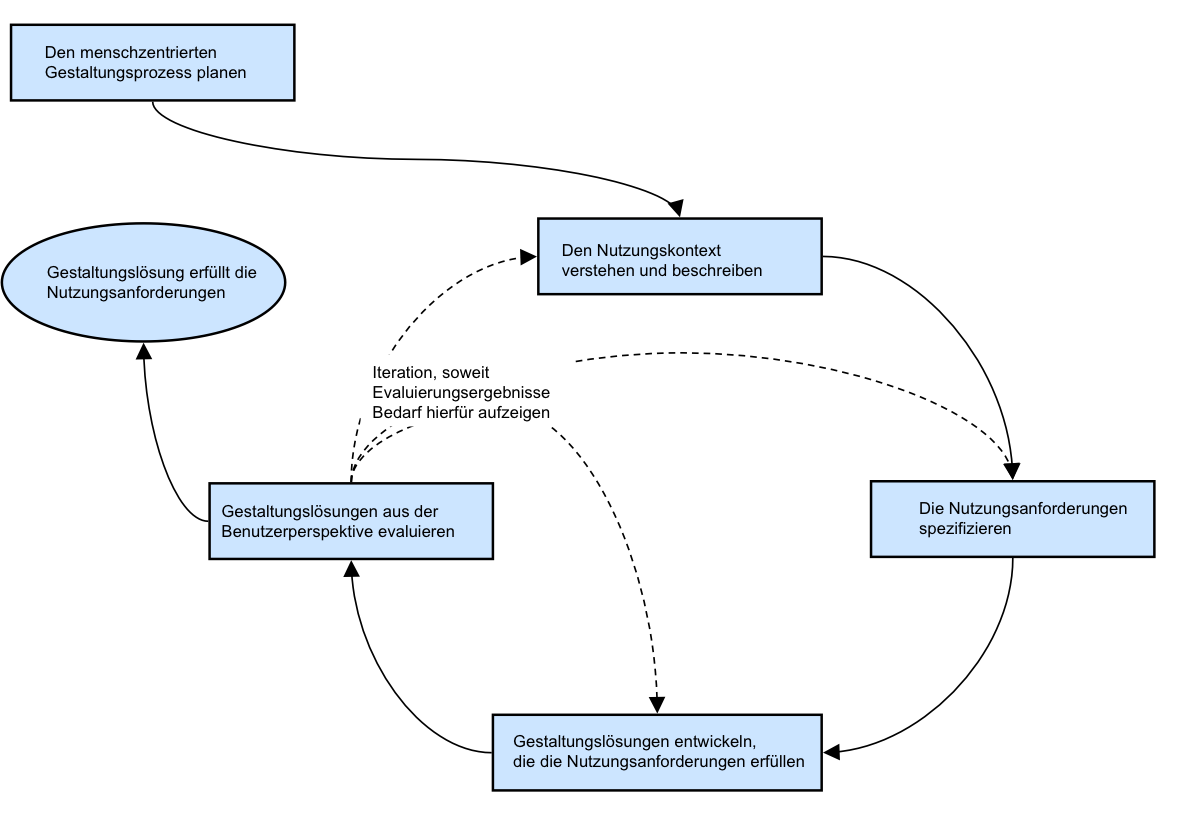
\includegraphics[width=10cm]{HCD.png}
\end{figure}

Das Schaubild der Iso Norm verdeutlicht den Ablauf eines Designprozesses in
mehreren Phasen. Nachdem geplant ist, was für ein Projekt umgesetzt werden soll
beginnt der zyklische Kreislauf des Entwicklungsprozesses. Im ersten Schritt
liegt der Fokus auf dem Analysieren der Situation, in der das zu entwickelnde
System später eingesetzt werden soll. Nur wer den Kontext eines interaktiven
Systems kennt, kann die Schnittstelle zwischen Maschine und Mensch adäquat
gestalten. Im zweiten Schritt geht es darum aus den geplanten Erwartungen an
das System und der Analyse des Nutzungskontextes konkrete Anforderungen zu
formulieren. Hierbei geht es noch nicht nicht darum, wie diese Anforderungen
technisch umgesetzt werden könnten, sondern darum, welche Anforderungen das
fertige System überhaupt erfüllen soll. Im dritten Schritt geht es nun darum
diese Anforderungen tatsächlich umzusetzen und technische Lösungen zu
implementieren. Gibt es erste Ergebnisse wird der vierte Schritt relevant: Die
Umgesetzte Lösungen müssen im tatsächlichen Nutzungskontext evaluiert werden.
Das setzt wieder eine intensiven Austausch mit den Nutzenden des Systems
voraus. Mit dem so gewonnen Feedback kann der Prozess wieder von vorne
beginnen. Fehlende Features können nachgebessert, missverständliche
Schnittstellen klarer gestaltet und Probleme im praktischen Einsatz minimiert
werden.\cite{iso9241}

G.A. Boy berichtet in \glqq{}The Handbook of Human-Machine Interaction\grqq{}
wie wichtig es ist, dem späteren Nutzenden der System erste Prototypen und
Ideen zu präsentieren. Oftmals wissen die Nutzenden gar nicht welche
technischen Möglichkeiten es gibt oder welche alternativen Bedienkonzepte in
ihrem Kontext besonders gut funktionieren könnten. Neben dem Zuhören und
Eingehen auf die Nutzenden und ihr Umfeld ist also auch das Einbringen und zur
Diskussion stellen neuer, für die Nutzenden unbekannter Lösungsansätze, von
hoher Bedeutung.\cite{HMI-HCD}

\section{Interview im Kontext}

Ein wesentlicher Bestandteil im Entwicklungsprozess nach den Methoden des Human
Centered Design ist der intensive Austausch mit den Nutzenden der Systeme.
Hierfür ist es wichtig, dass Softwareentwickler und Designer von
Benutzerschnittstellen in den direkten Austausch mit den Nutzenden der Systeme
gehen. Um diesen Prozess strukturiert und zielführend zu durchlaufen, kann
hierfür die Methode des \textbf{Interviews im Kontext} benutzt werden.

Beim Interview im Kontext geht es darum, die Nutzenden der Systeme in dem
Umfeld zu beobachten, in dem die Software tatsächlich auch im praktischen
Alltag eingesetzt wird. Der Fokus liegt also auf dem Umfeld der Interaktion mit
technischen Systemen. In herkömmliche Interviews begegnen sich Interviewer und
Interviewter oftmals in einer neutralen Umgebung, wie beispielsweise einem
Konferenzraum und sprechen über die Prozesse für die sich der Interviewende
interessiert. Beim Interview im Kontext geht es nicht darum \textbf{über} einen
Prozess zu sprechen, sondern den Prozess als Interviewender \textbf{direkt
    mitzuerleben}.\cite{contextualDesign} In \textit{Manual on Human-Computer
    Interaction} legen die Autoren den Fokus auf die genaue Beobachtung der
NuTzenden in der Interaktion mit den Systemen. Mit dieser Methode könne man
noch viel mehr praxisnahe Details erfassen, als wenn man mit den Nutzenden nur
über das System spricht. Spricht man mit Nutzenden beispielsweise darüber wie
sie eine Software bedienen, gibt es möglicherweise viele Dinge, die sie nicht
erwähnen, weil sie vergessen wurden, nicht relevant erscheinen oder Nutzende
nicht wissen, wie sie genau darüber sprechen sollen.\cite{hciHandbook}

Dies kann in der Praxis bedeuten, dass man sich mit den Nutzenden der Systeme
in ihren Büroräumen trifft und für mehrere Stunden mit dabei ist, wenn sie
ihrer Arbeit nachgehen und mit den technischen Systemen interagieren. Die Rolle
des Interviewenden ist dabei aus einer beobachtenden Perspektive zu verstehen.
Der Interviewte soll die Richtung bestimmen, in die sich das Interview
entwickelt. Der Interviewende hört hauptsächlich zu und beobachtet wie die
Personen in ihrer Umgebung, ihrem Kontext agieren.\cite{hciHandbook} Dazu kann
der Interviewende Notizen machen um eine spätere Auswertung des Interviews zu
erleichtern. An passenden Stellen kann der Interviewende gezielte Nachfragen
stellen um beispielsweise Hürden bei der Interaktion mit den Systemen zu
provozieren. Eine weitere Intention für Nachfragen kann aber auch sein, die
Gedanken und Emotionen des Nutzenden zu erfragen, welche er beim Benutzen des
Systems empfindet.

\begin{figure}[h]
    \caption{Während eines Interviews im Kontext können viele Aspekte beobachtet werden die über das benutzte System selbst hinausgehen\cite{johannesGrafik}}
    \centering
    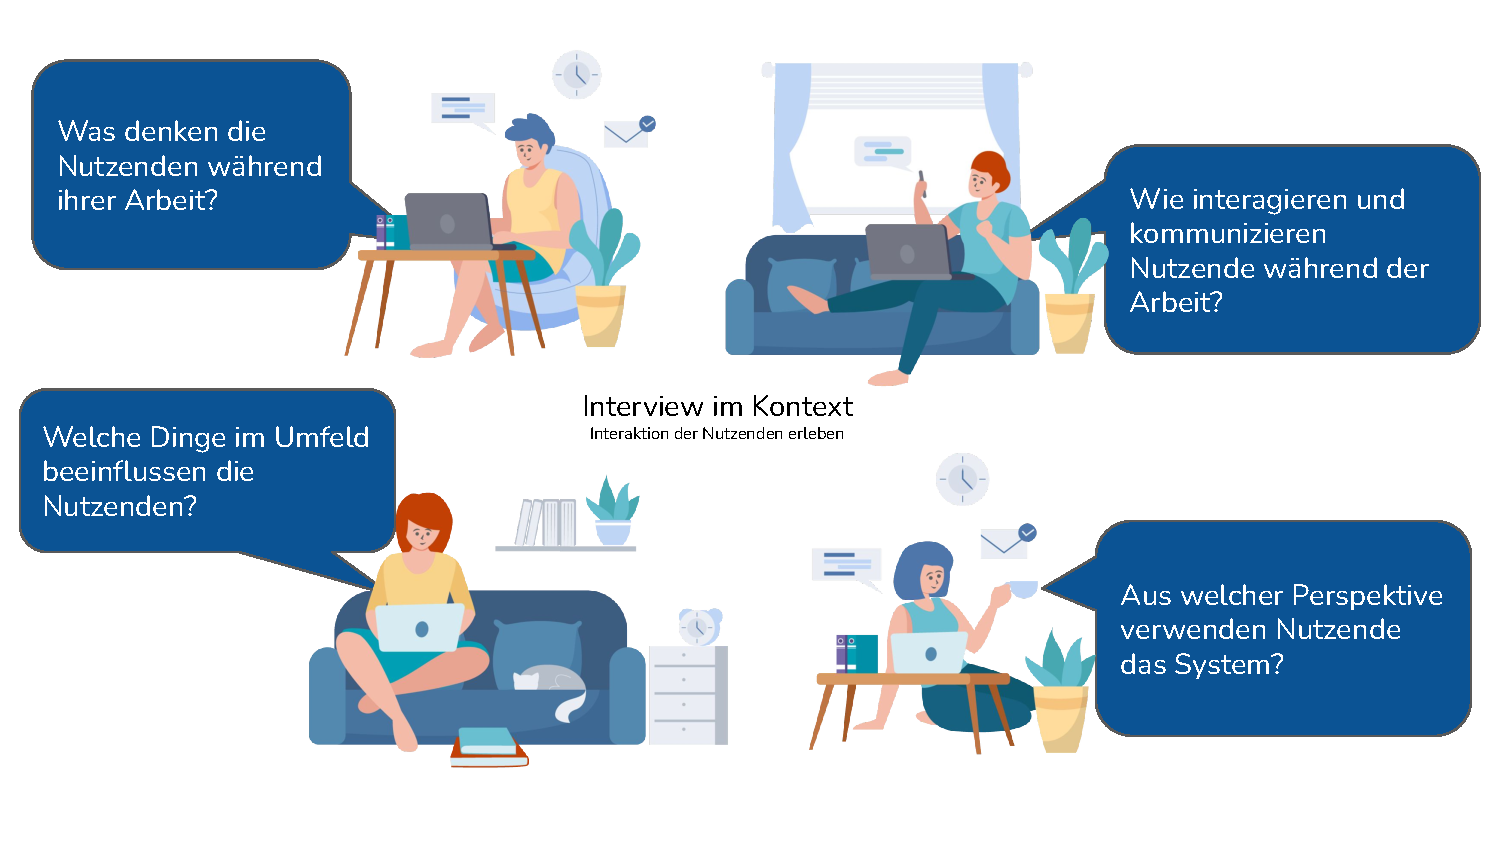
\includegraphics[width=0.9\textwidth]{Interview im Kontext Schaubild.pdf}
\end{figure}

Das Ergebnis eines Interviews im Kontext ist also eine ausführliche Beobachtung
der Interaktion von Nutzenden mit den entsprechenden Systemen im alltäglichen
Kontext. Diese Beobachtungen können schriftlich festgehalten werden oder auch
durch Video- und Tonaufzeichnungen ergänzt werden. Im Nachgang des Interviews
müssen die Beobachtungen ausgewertet und analysiert werden. Ziel ist es dabei
aus den Beobachtungen des Interviews konkrete Nutzungsanforderung an das zu
entwickelnde System zu formulieren. Hier können beispielsweise Featurelisten,
Diagramme oder User-Scenarios zum Einsatz kommen.\cite{HMI-HCD}
\section{Durchführung}

\subsection{Situation in der Abteilung}

\paragraph{Überleitung Situation Abteilung}
Um den Bedarf und Entstehungsprozess der Software besser einordnen zu können,
werden nun die Workflows und Prozessabläufe im Büroteam kurz skizziert. Die
Beschreibung der Situation im Team hilft zu erkennen, wie sich die aktuelle
Softwarelösung in den Arbeitsalltag eingliedert, welche Prozessabläufe bereits
gut durch Software begleitet werden, und an welchen Stellen noch
Optimierungsbedarf besteht.

\paragraph{Grundlegende Beschreibung der Abteilung}
Als Nutzergruppe aller Studien dieser Bachelorarbeit werden die Mitarbeitenden
einer Abteilung der Hochschulverwaltung an der Universität Kassel dienen. Es
handelt sich um die Abteilung "Studium und Lehre", zu deren alltäglichen
Aufgaben es gehört, alle erdenklichen Organisationen zu übernehmen, die
Studierenden und Lehrenden ein erfolgreiches Zusammenarbeiten an der
Universität ermöglichen. Hierzu gehören beispielsweise das Einschreiben, und
Exmatrikulieren von Studierenden, die Durchführung des Bewerbungsverfahrens,
das Betrieben der Information Studium und die allgemeine Studienberatung. In
dieser Arbeit wird der Fokus auf die Mitarbeitenden der Studienberatung in der
Abteilung Studium und Lehre gesetzt.

\paragraph{Studienberatung}
Die allgemeine Studienberatung der Universität Kassel berät Studierende zu
allen Fragen rund um das Studium. Insbesondere bei persönlichen Problemen mit
der Fertigstellung des eigenen Studiums hilft die Studienberatung mit einem
persönlichen Lösungsgespräch und kann an weitere fachspezifische
Beratungsstellen weiter vermitteln. Des Weiteren bietet die allgemeine
Studienberatung verschiedene Workshops und Seminare an. Hierbei können sich
Studierende in Gruppen mit Fokus auf bestimmten Fragestellungen austauschen und
Qualifikationen im Umgang mit herausfordernden Studiensituationen erlangen.
Auch "Schnupperkurse" für Studieninteressierte und Schüler werden von der
allgemeinen Studienberatung angeboten um jungen Menschen mit Interesse an einem
Studium einen möglichst unmittelbaren Einblick in den Studienalltag zu
gewähren.\cite{studBeratungKsWeb}

\paragraph{Terminvereinbarung in der ZSB}
Eines der zentralen Themen im Alltag der Studienberatung sind Beratungstermine.
\todo{gendern?} Studienberatende müssen Termine mit den Ratsuchenden
vereinbaren und abstimmen. Beratungstermine können über verschiedene
Kontaktkanäle stattfinden: Es ist eine telefonische Beratung oder auch eine
Beratung über eine Videokonferenz möglich. Selbstverständlich ist auch möglich
einen persönlichen Beratungskontakt vor Ort zu vereinbaren. Über all diese
Termine muss jeder Studienberatende den Überblick behalten und gleichzeitig
neue Terminanfragen schnell beantworten können. Um diesen Prozess zu
erleichtern und mögliche Fehler, wie beispielsweise Terminüberschneidungen, zu
minimieren, wird hierfür die \textbf{Software "Stubegru"} eingesetzt.

\subsection{Aktuelle Softwarelösung}
\paragraph{Stubegru}
Stubegru ist ein umfangreiches Softwarepaket für akademische Beratungsstellen.
Die webbasierte Groupware begleitet viele Arbeitsabläufe im Alltag einer
Beratungsstelle an einer Hochschule. In einem Softwaresystem vereint Stubegru
eine Wissensdatenbank in Form eines Wikis, sowie ein Dashboard mit vielen
Modulen für spezifische Workflows. So können über Stubegru an der Universität
Kassel beispielsweise Abwesenheiten der Abteilung, Telefonnotizen und
Beratungskontakte verwaltet werden. Jeder Mitarbeitende der Abteilung hat über
einen eigenen Account Zugriff auf die Software, die er im Browser aufrufen
kann. Die Software hilft dabei tagesaktuelle Informationen schnell und
übersichtlich allen Mitarbeitenden zur Verfügung zu stellen und bei Bedarf
langfristige und ausführliche Informationen mit wenigen Klicks zur Verfügung zu
stellen.\cite{stubegruWebsite}

\paragraph{Terminvereinbarung in Stubegru}
Das wichtigste Modul der eingesetzten Software für die Studienberatung ist der
Kalender zur Terminvereinbarung von Beratungsterminen. Über diese Modul können
in einem zweistufigen Prozess Termine für Ratsuchende freigegeben und an die
entsprechenden Studierenden und Studieninteressierten vermittelt werden.

\paragraph{Zeitslots erstellen}
Im ersten Schritt können die Studienberatenden freie Zeitslots für ihre
Beratungstermine anlegen. Diese Zeitslots zeigen an, dass der entsprechende
Beratende in der eingestellten Zeitspanne potenziell Zeit für ein
Beratungsgespräch hat. Bei der Erstellung der Zeitslot können weitere Attribute
wie der Beratungskanal (Online Meeting, Telefongespräch oder Präsenztermin)
konfiguriert werden. Außerdem können Mail Templates verknüpft werden, die im
Falle einer Terminvergabe den Ratsuchenden per Email über alle wichtigen
Informationen zum Termin informieren.

\paragraph{Terminvergabe durch Erstinformation}
Im zweiten Schritt werden die eingestellten Zeitslots durch Hilfskräfte der
Erstinformation an Ratsuchende vergeben. Die Erstinformation der Universität
Kassel berät Studierende und Studieninteressierte zu allen Fragen rund ums
Studium übers Telefon, Email und eine Servicetheke vor Ort. Bei tiefgehenden
Fragen und spezifischen Anliegen verweisen die Mitarbeitenden an die
entsprechenden Sachbearbeitenden oder Beratungsstellen. Die Erstinformation ist
auch für das vereinbaren von Beratungsterminen mit der allgemeinen
Studienberatung verantwortlich. Sind die Mitarbeitenden der Erstinformation in
Kontakt mit einem Kunden, der einen Termin in Anspruch nehmen möchte, können
sie in der Software alle freien Zeitslots der Beratenden einsehen und einen
passenden Termin mit den Kunden vereinbaren. Wenn ein freier Zeitslot vergeben
wird und fest mit einem Ratsuchenden verknüpft ist, wird eine Email an den
Beratenden versendet, der über alle Details wie Adresse, Kontaktinformationen
und Anliegen der Ratsuchenden informiert wird. Des Weiteren wird eine Mail an
die Ratsuchende Person versendet, die auf dem zuvor verknüpften Mailtemplate
aufbaut und dynamisch terminrelevante Informationen einsetzt, wie
beispielsweise Datum und Zeit des Termins, oder eine Wegbeschreibung zum
Beratungsraum.

\paragraph{Auskunft bei Terminabsage}
Eine weitere Verwendung des Kalendermoduls tritt ein, wenn Kunden der
Erstinformationen Fragen zu einem bereits vereinbarten Termin haben oder diesen
Absagen möchten. In diesem Fall können die Hilfskräfte der Erstinformation über
eine Suchfunktion gezielt nach den vereinbarten Terminen des Kunden suchen und
weitere Auskünfte geben.

\paragraph{Datenschutz}
Da Datenschutz in Beratungsszenarien eine wichtige Rolle einnimmt, kann
lediglich der verantwortliche Beratende das Anliegen der ratsuchenden Person
einsehen. Zu Auskunftszwecken können aber alle Mitarbeitenden der Abteilung
sehen, wann ein Beratungstermin mit welchem Beratenden vereinbart wurde.
Datensätze zu vergangenen Beratungstermin werden täglich gelöscht, sodass
möglichst wenig personenbezogenen Daten in der Datenbank gespeichert werden
müssen. Über ein differenziertes Berechtigungssystem der eingesetzten Software
Stubegru, kann genau gesteuert werden, welche Nutzergruppen Beratungstermine
anlegen und vergeben dürfen.

\subsection{Grund für Veränderung}

\paragraph{Neue Softwareversion}
Die Software Stubegru wurde ursprünglich von einer Hilfskraft der Abteilung
Studium und Lehre an der Universität Kassel erstellt und betreut. Da die
Software nun langfristig an der Uni Kassel und auch an anderen deutschen
Hochschulen eingesetzt werden soll, wurde ein Prozess gestartet, um eine
Professionalisierung und nachhaltige Betreuung der Software zu gewährleisten.
In diesem Rahmen wurde die Software auch für andere Hochschulen zur Verfügung
gestellt und unter einer OpenSource Lizenz veröffentlicht. Im Zuge dieser
Veröffentlichung wurde in Zusammenarbeit mit der Hochschule Bremen eine
grundlegend überarbeitete Variante der Software Stubegru erstellt, die im
Vergleich zu der bisherigen Version deutlich flexibler ist und mehr
Anpassungsmöglichkeiten bietet. Wie Erich Gamma in \textit{Elemente
    wiederverwendbarer objektorientierter Software} betont, bieten wiederverwendbar
gestaltete Softwarestrukturen und abstrakte Implementierungsansätze die Option,
Softwaremodule in verschiedenen Kontexten zu verwenden. Dies erfordert im
Softwareentwurf allerdings eine vorausschauende Planung und einen hohen
Abstraktionsgrad.\cite{wiederverwSoftware} Somit ist der Einsatz der Software
Stubegru an verschiedenen Hochschulen mit verschiedenen Arbeitsabläufen
realisierbar. Um von dieser neuen, überarbeiteten Softwareversion auch an der
Universität Kassel zu profitieren, ist wiederrum eine grundlegende
Überarbeitung des Moduls zur Terminvergabe der Beratungstermine für die
allgemeinen Studienberatung notwendig.

\paragraph{Fehlende Features}
In der aktuellen Softwareversion gibt es einige Features, die noch nicht
vollständig funktionieren oder nicht optimal auf den tatsächlichen
Arbeitsalltag zugeschnitten sind. An diesen Stellen soll das neue Modul zur
Terminvereinbarung verbessert und noch weiter an die Bedürfnisse der Nutzenden
angepasst werden. Im Rahmen der Softwareüberarbeitung mit der Hochschule Bremen
wurde für die neue Version von Stubegru bereits ein Kalendermodul zur Vergabe
von Beratungsterminen entwickelt. Dieses Modul weist allerdings noch einige
Probleme auf, um reibungslos im Arbeitsalltag der allgemeinen Studienberatung
an der Universität Kassel eingesetzt zu werden. In der "Bremer Version" läuft
das Erstellen und Vergeben eines Beratungstermins in einem einzigen Schritt ab.
Ein zentraler Punkt um die überarbeitete Software auch in der allgemeinen
Studienberatung der Universität Kassel nutzen zu können ist der zweistufige
Prozess der Terminvergabe. Hier müssen Beratende die Möglichkeit haben zuerst
freie Terminslots freizugeben, die dann in einem getrennten zweiten Schritt
durch Mitarbeitende der Erstinformation an Ratsuchende vergeben werden können.

\paragraph{Vorschau auf Hauptteil der Arbeit}
Welche Anpassungen im Detail notwendig sind, um die Software optimal in der
Studienberatung einsetzen zu können, soll in den folgenden Kapiteln methodisch
herausgearbeitet werden und durch Dokumentation von praktische durchgeführten
Nutzerstudien und Gesprächen mit den verantwortlichen Personen ergänzt werden.
Diese Bachelorarbeit soll insbesondere den Designprozess strukturiert begleiten
und wissenschaftliche Methoden aufzeigen, um Softwareentwicklern und Nutzenden
eine möglichst gute Zusammenarbeit zu ermöglichen.

\subsection{Nutzungskontext verstehen - Interview im Kontext}

\paragraph{Warum Interview im Kontext?}
Das Modul zur Terminvereinbarung der Software Stubegru soll auf den
Arbeitsalltag der allgemeinen Studienberatung der Universität Kassel angepasst
werden. Dies soll mit Methoden des Human Centered Design umgesetzt werden. Ein
zentraler Bestandteil des Human Centered Design ist der enge und stetige
Austausch mit den Nutzenden des Softwaresystems \cite{hci} \todo{Quelle
    checken} Um den Änderungsbedarf eines bestehenden Softwaresystems einschätzen
zu können wird im Human Centered Design häufig die Methode des
\textit{Interviews im Kontext} gewählt.\cite{contextualDesign} Diese Methode
eignet sich besonders zu Beginn des Entwicklungsprozesses, da wenig
Vorkenntnisse über die eingesetzte Software und das Umfeld, in dem Software
eingesetzt wird, bekannt sein muss. Die Softwareentwickler können so einen
guten Einstieg finden, um einen Überblick zu gewinnen, welche Funktionen die
fertige Software am Ende unterstützen muss. Auch lässt sich durch ein genaues
Beobachten beim Interview herausarbeiten, in welchem Kontext die Software im
tatsächlichen Arbeitsalltag genutzt wird und welche weiteren Faktoren die
Nutzenden der Systeme beeinflussen.

\subsubsection{Kontext des Interviews}

\paragraph{Rahmenbedingungen IiK}
Als erster Schritt wurde ein Termin für ein Interview im Kontext mit \ipName
\todo{Anonymisierung angeben?} vereinbart. \ipName ist einer von drei
Mitarbeitenden der allgemeinen Studienberatung der Universität Kassel. Zu
seinen Aufgaben gehört die Betreuung der Software Stubegru und deren Einsatz in
der Abteilung Studium und Lehre. Seit über sechs Jahren arbeitet \ipName
bereits gemeinsam mit Hilfskräften an dem Aufbau und der Optimierung der
Software Stubegru um den täglichen Arbeitsalltag seines Teams optimal zu
unterstützen. Ich habe mich persönlich mit \ipName in seinem Büro im Campus
Center der Universität getroffen. Dort hat er mir an seinem Schreibtisch
gezeigt, wie er mit der alten Version der Software Beratungstermine erstellt
und vergeben kann. \ipName saß vor mir und hatte Maus und Tastatur in der Hand.
Ich saß hinter ihm auf einem Stuhl und habe auf einem iPad Notizen
mitgeschrieben. Für die Dauer von einer Stunde hat \ipName mir gezeigt, wie er
die Software aktuelle nutzt, welche Features für ihn sehr wichtig sind und an
welchen Stellen noch Verbesserungspotenzial besteht.

\paragraph{Detaillierter Ablauf IiK}
Am Anfang habe ich \ipName gebeten, mir einmal zu zeigen, wie er einen
Beratungstermin in der Software anlegen und vergeben kann. Dies ist der
Workflow, der im Arbeitsalltag am häufigsten vorkommt und daher eine hohe
Priorität im Designprozess hat. \ipName klickte sich durch die verschiedenen
Eingabefelder um einen freien Zeitslot für einen Beratungstermin anzulegen.
Hierbei erwähnte er, dass es ganz wichtig ist, dass Datum und Uhrzeit des
Beratungstermins mit wenigen Klicks über ein Date-/Timepicker mit der Maus
eingeben werden können. Eine Datumseingabe über die Tastatur würde er nicht
bevorzugen.

\begin{figure}[h]
    \caption{Datepicker im Formular zur Erstellung eines Zeitslots}
    \centering
    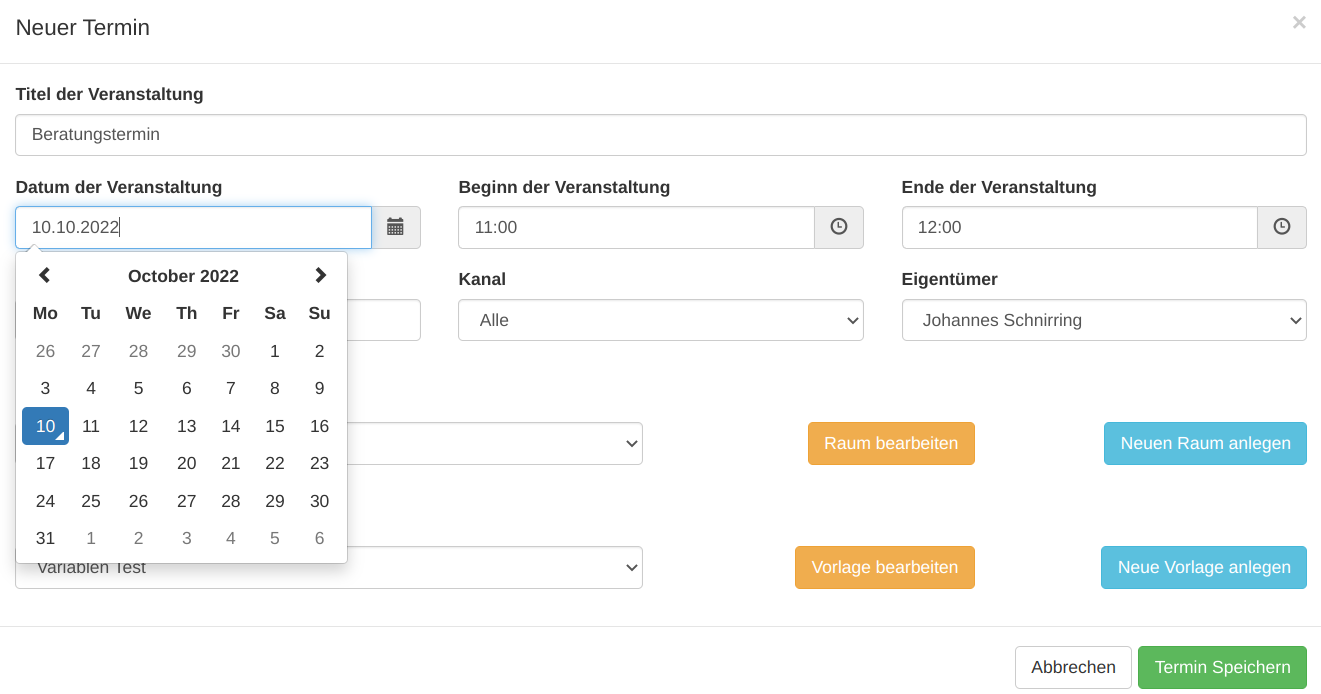
\includegraphics[width=0.9\textwidth]{screen_old_datepicker.png}
\end{figure}

Beim Eintragen mehrere Termine wäre es auch besonders praktisch, dass das zuvor
eingegebene Datum stehen bleibt und direkt ein weiterer Zeitslot für den
gleichen Tag angelegt werden kann, ohne dass er nochmal extra das Datum
auswählen muss. Diem meisten der weiteren Felder sind Dropdown Menüs, mit
wenigen Elemente., Die Auswahl der richtigen Werte kann \ipName schnell
vornehmen. Bei der Auswahl der verknüpften Räume werden beispielsweise die
Räume, die mit seinem Nutzeraccount verknüpft sind, ganz oben in der
Auswahlliste angezeigt. Da eine Beratung in der Regel in den eigen Räumen
stattfindet, ist hier eine schnelle Auswahl für den Normalfall möglich. In
einer Spezialsituation, in der ein größerer Beratungstermin beispielsweise in
einem gemeinsamen Gruppenraum stattfinden, ist aber auch solch eine Auswahl
möglich.

\begin{figure}[h]
    \caption{Dropdown zur Auswahl des Beratungsraums. Der eigene Raum wird immer als oberstes angezeigt}
    \centering
    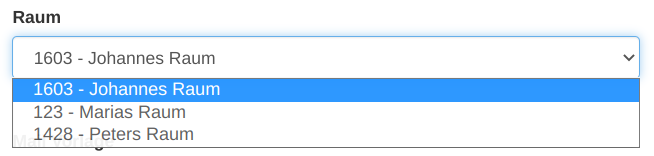
\includegraphics[width=0.9\textwidth]{screen_old_roomdropdown.png}
\end{figure}

Nachdem der Zeitslot für den Termin angelegt ist, wird der entsprechende Tag in
der Kalenderübersicht nun grün hinterlegt. Dies ist ein Zeichen für die
Hilfskräfte der Erstinformation, dass an diesem Tag noch freie Zeitslots
verfügbar sind.

\begin{figure}[h]
    \caption{Kalenderübersicht. Grüne gefärbte Tage zeigen noch freie Zeitslots an. Rot gefärbte Tage weisen auf vergeben Zeitslots hin}
    \centering
    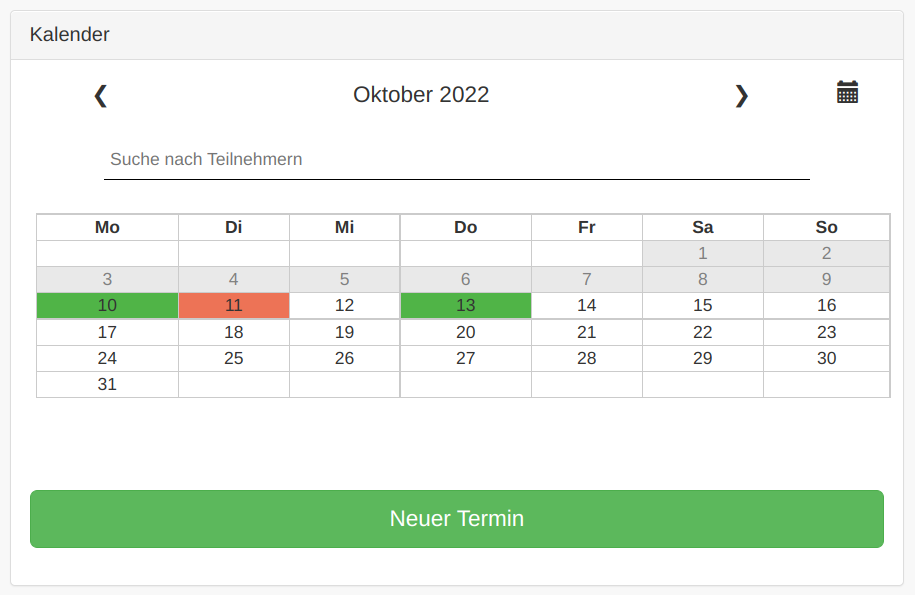
\includegraphics[width=0.9\textwidth]{screen_old_module.png}
\end{figure}

Durch ein Mouseover über den entsprechenden Tag in der Monatsübersicht kann man
die genauen Termine mit Informationen über die Uhrzeit, den zuständigen
Beratenden und die Anzahl der freien Plätze sehen. \ipName erklärt mir, dass
die kompakte Monatsansicht mit den farblich hervorgehobenen Terminslots bereits
eine sehr gute Lösung ist, damit die Hilfskräfte auf einen Blick erfassen
können, an welche Tagen sie den Kunden noch Beratungsgespräche anbieten können.
Sobald alle Plätze der Beratungstermine an einem Tag vergeben sind, wird dieser
im Kalender rot markiert. \glqq So sehen Hilfskräfte mit einem Blick sofort,
dass sie hier keinen Termin mehr vergeben werden können\grqq, erklärt \ipName
\cite{claves}.

\begin{figure}[h]
    \caption{Bewegt man den Mauszeiger über einen Tag, erscheinen weiteren Informationen zu den Zeitslots an diesem Tag}
    \centering
    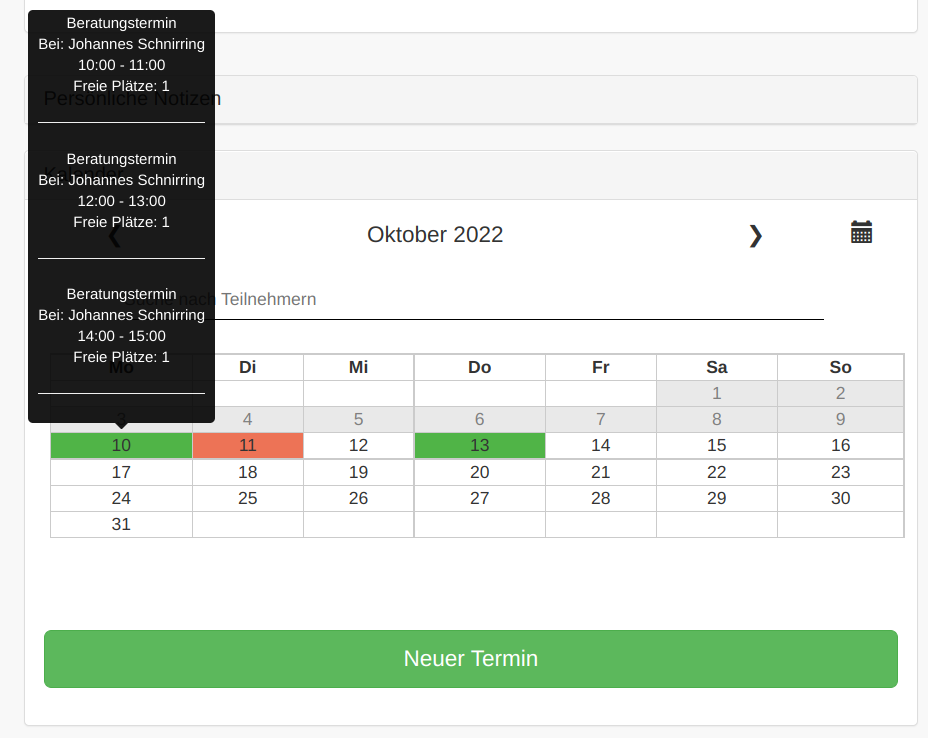
\includegraphics[width=0.9\textwidth]{screen_old_hover.png}
\end{figure}

Soll nun ein Zeitslot tatsächlich vergeben werden, klickt man auf den
entsprechenden Tag in der Monatsansicht und es öffnet sich ein Modal. Dies ist
ein Fenster, welches sich über den anderen Bildschirminhalt legt und dem Nutzer
somit deutlich anzeigt, dass hier eine Aktion im neu geöffnet Fenster notwendig
ist. \ipName zeigt mir, wie die Mitarbeitenden der Erstinformation in diesem
Detail-View die freien Zeitslots an die ratsuchenden Personen vergeben können.
In einer Liste werden, nach Uhrzeit sortiert, alle Termine untereinander
angezeigt. Neben jedem freien Termin steht ein Button zum Vergabe dieses
Zeitslots zur Verfügung.

\begin{figure}[h]
    \caption{Der Detail-View: Eine Liste mit drei freien Zeitslots am entsprechenden Datum}
    \centering
    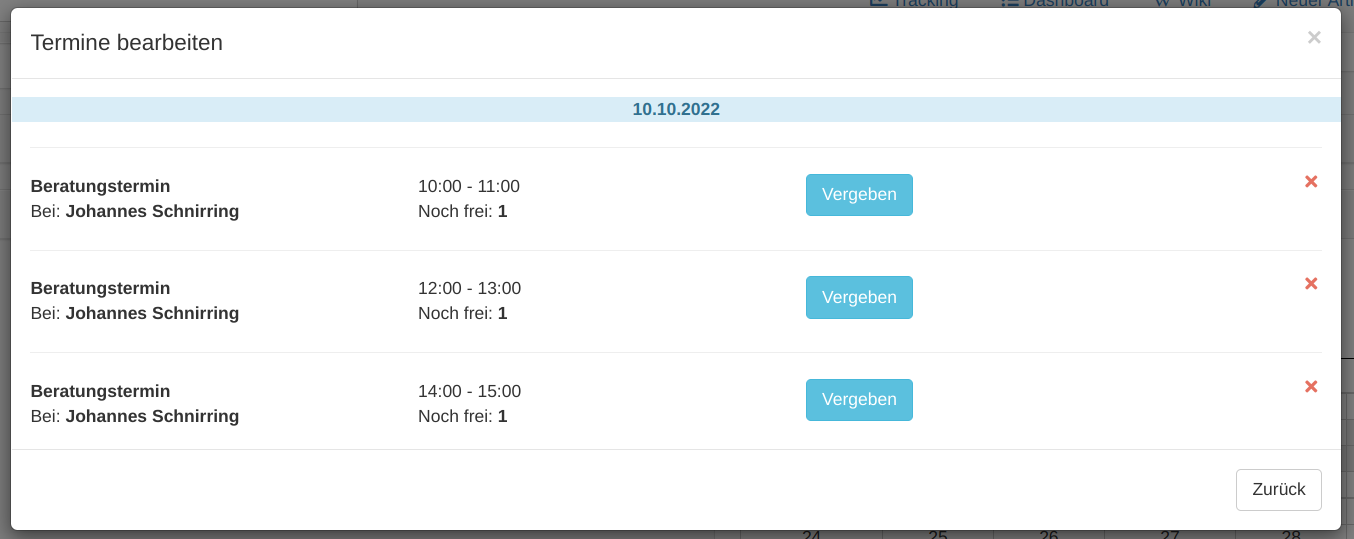
\includegraphics[width=0.9\textwidth]{screen_old_daylist.png}
\end{figure}

\ipName zeigt mir wie eine Hilfskraft der Erstinformation nun einen solchen
Zeitslot vergeben könnte. Nach Klick auf den "Vergabe-Button" klappt ein
Formular auf, indem Name, Kontaktdaten und Anliegen der Ratsuchenden erfasst
werden können.

\begin{figure}[h]
    \caption{Formular zum vergeben eines Zeitslots an eine ratsuchende Person}
    \centering
    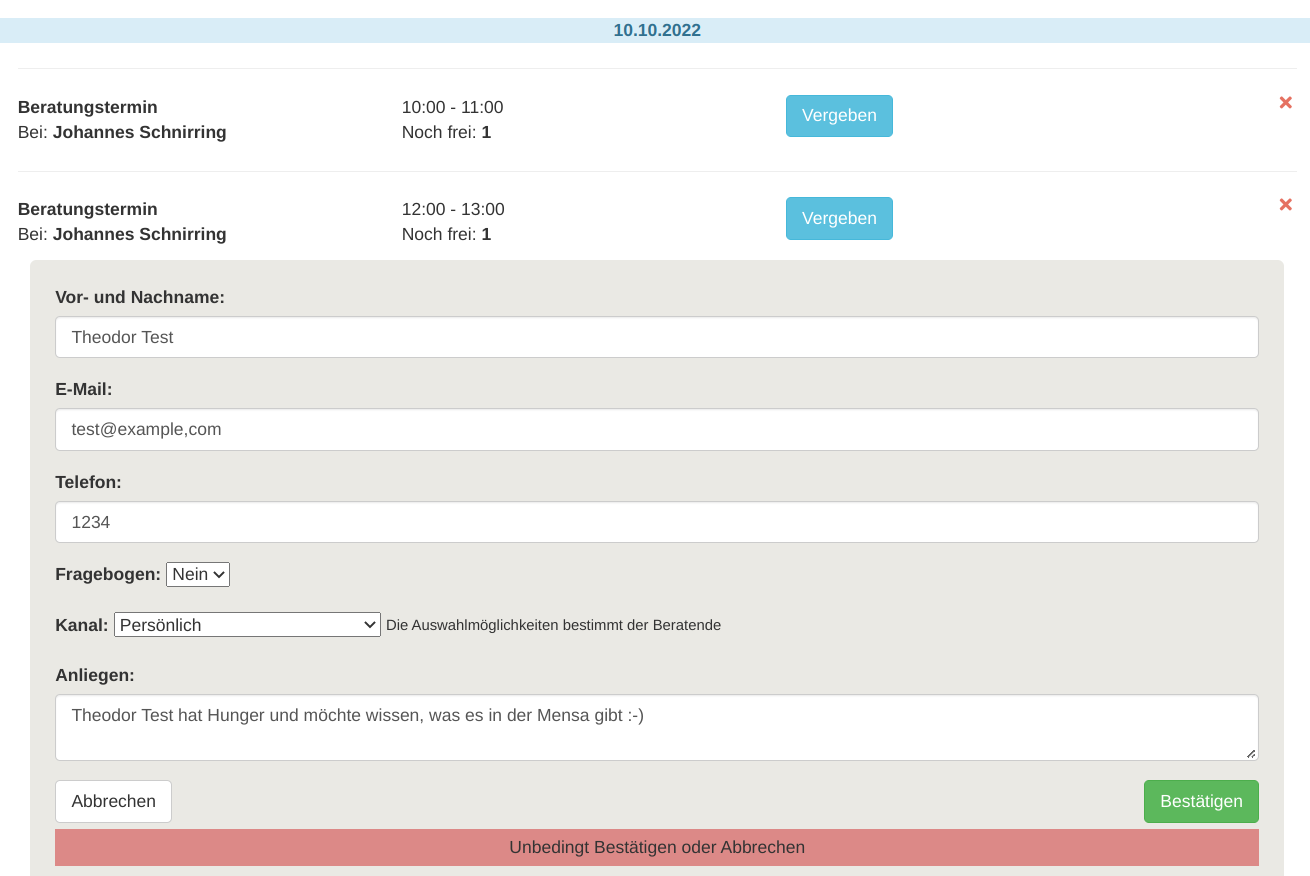
\includegraphics[width=0.9\textwidth]{screen_old_clientdata.png}
\end{figure}

Nachdem alle personenbezogenen Daten korrekt erfasst wurden kann der Termin nun
endgültig gebucht werden. Hierzu klicken die Hilfskräfte auf den Button
"Bestätigen". \ipName erklärt mir, dass dies ein sehr wichtiger Schritt ist:
Solange eine Mitarbeitender der Erstinformation das Formular zum Erfassen der
persönlichen Daten des Ratsuchenden geöffnet hat, wird dieser Zeitslot mit
einer Sperre versehen. So wird verhindert, dass dieser Zeitslot von einem
Kollegen vergeben werden kann, während man selbst gerade mit dem Ratsuchenden
beispielsweise am Telefon die persönlichen Daten und das Anliegen bespricht.
Sollte nach dem Aufklappen des Formulars der entsprechende Zeitslot doch nicht
vergeben werden, ist es deshalb notwendig, dass die terminvergebende Person auf
"Abbrechen" klickt, um die Sperre dieses Zeitslots aufzuheben und ihn somit für
die Kollegen wieder freizugeben. \ipName betont, dass dieser Schritt manchmal
nicht ganz intuitiv ist, und für die Hilfskräfte daher in Einführungsschulungen
immer besonders hervorgehoben wird. Es wäre allerdings deutlich schlimmer einen
Termin doppelt zu vergeben und somit mindestens einer ratsuchenden Person
wieder absagen zu müssen, als einen Zeitslot versehentlich zu sperren.

\begin{figure}[h]
    \caption{Detail-View: Ein Zeitslot wurde nun vergeben und ist für den entsprechenden Kunden reserviert. Hilfskräfte können nur den Namen des Ratsuchenden einsehen}
    \centering
    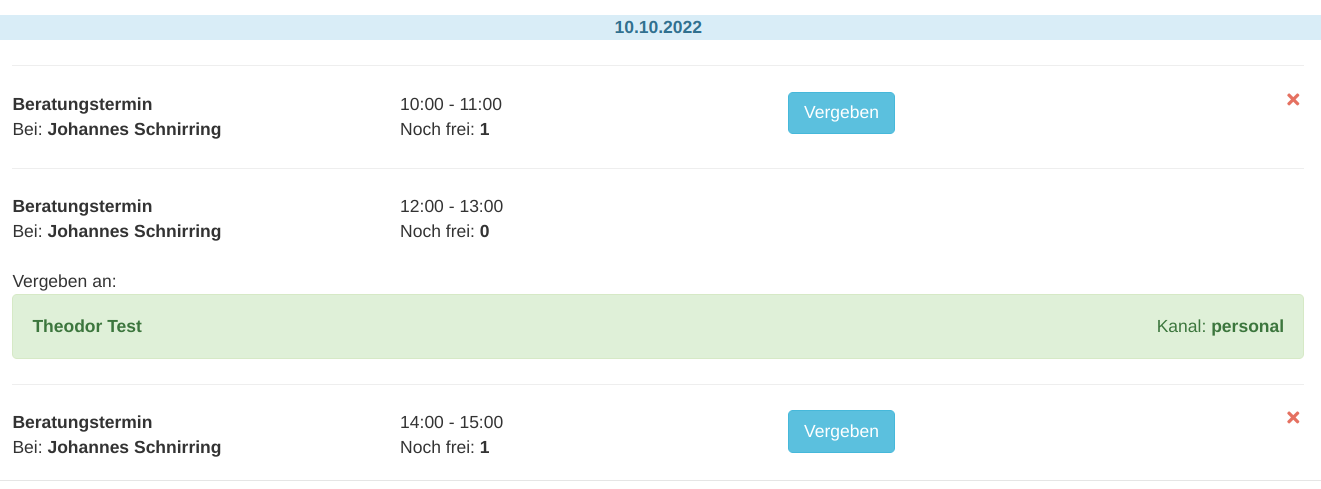
\includegraphics[width=0.9\textwidth]{screen_old_assigned_hiwi.png}
\end{figure}

Ist der Termin nun erfolgreich vergeben, können alle Nutzenden der Software
einsehen an welche Person dieser Termin vergeben wurde. Meldet sich ein
Ratsuchender beispielsweise einige Tage später noch einmal bei der
Erstinformation und möchte wissen, wann sein Beratungstermin stattfindet,
können die Mitarbeitenden der Erstinformation diese Auskunft aus der Software
ablesen. Aus Datenschutzgründen können allerdings keine weiteren
personenbezogenen Daten des Beratungstermins ausgelesen werden. Lediglich der
Studienberatende, bei dem der Termin stattfindet, bekommt beim Aufruf des
Detail-Views weitere Details wie Kontaktdaten und Anliegen der ratsuchenden
Person angezeigt.

\begin{figure}[h]
    \caption{Detail-View: Der verantwortliche Beratende kann weitere personenbezogene Details einsehen}
    \centering
    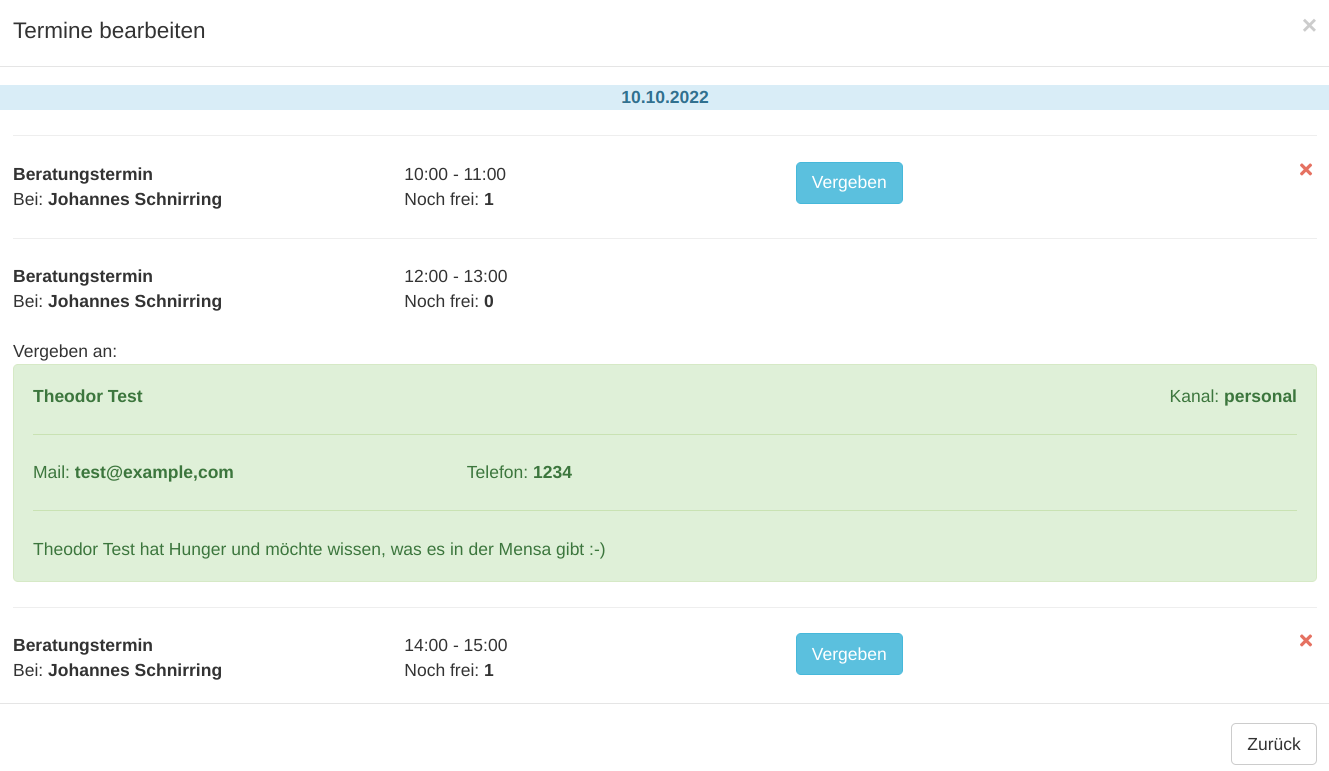
\includegraphics[width=0.9\textwidth]{screen_old_assigned.png}
\end{figure}

\ipName hat nun den zweistufigen Workflow zur Terminvergabe einmal komplett
durchgespielt und mich auf viele Details hingewiesen. Während \ipName mir
gezeigt und erzählt hat, wie die Terminvergabe in der aktuellen Softwareversion
abläuft, habe ich in Stichworten mitgeschrieben, welche Bemerkungen und
Auffälligkeiten er besonders betont hat.

\subsubsection{Auswertung des Interviews}

\paragraph{Einleitung Auswertung}
Während bisher der detaillierte Ablauf des Interviews im Kontext geschildert
wurde, sollen im Folgenden die wesentlichen Kernaspekte nochmals
zusammengefasst werden, die während des Interviews notiert wurden. Das
Augenmerk liegt hierbei auf Beobachtungen, die Konsequenzen für den
Designprozess des überarbeiteten Kalendermoduls zur Terminvergabe
hervorbringen.

\paragraph{Methode der Auswertung}
Während dem Interview habe ich mir alle relevant erscheinenden Aussagen von
\ipName auf einem iPad notiert. Wurden im weiteren Gesprächsverlauf noch
ergänzenden Informationen zu den einzelnen Punkten deutlich, habe ich diese in
den Notizen stichpunktartig an die entsprechenden Themen angefügt. Im Nachgang
des Interviews mussten diese Notizen nun sorgfältig analysiert und ausgewertet
werden. Hierzu bin ich die einzelnen Themen durchgegangen und habe die
entsprechenden Ansichten und Klickpfade in der Software nochmals nachgespielt.
In einem neuen Dokument habe ich nun die herausgearbeiteten Problematiken
zusammengefasst um die zu Grunde liegenden Zusammenhänge klarzustellen und zu
spezifizieren. Dies entspricht dem zweiten Schritt des iterativen Design Zyklus
des Human Centered Design nach ISO 9241 \cite{iso9241}

\paragraph{Spannende Erkenntnisse}
Im Folgenden werden nun drei Punkte exemplarisch vorgestellt, die während des
Interviews aufgefallen sind. Anhand dieser drei verschiedenen bestehenden
Probleme wird der Designprozess des Human centered Design beispielhaft
durchlaufen.

\paragraph{Kompakte Ansicht Kalender (mit Farben)}
In der alten Softwareversion, die an der Uni Kassel bisher zum Einsatz kam,
werden alle freien und vergeben Zeitslots der Beratungstermine in einer
tabellarischen Monatsansicht dargestellt.

\begin{figure}[h]
    \caption{Tabellarische Ansicht der Zeitslots mit Einfärbungen der einzelnen Tage}
    \centering
    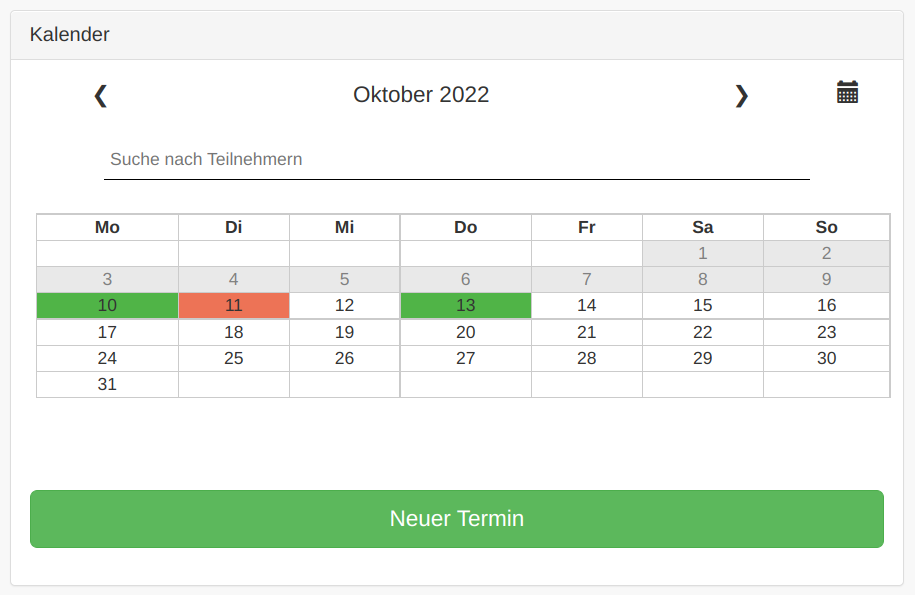
\includegraphics[width=0.9\textwidth]{screen_old_module.png}
\end{figure}

Durch die farblichen Markierungen der einzelnen Tage können Nutzenden auf einen
Blick erfassen, ob an diesem Tag Beratungsslots eingetragen wurden und ob unter
den eingetragenen Zeitslots noch freie Termine vorhanden sind. Ein grün
markierter Tag bedeutet, dass an diesem Tag noch mindestens ein freier
Beratungsslot vorhanden ist. Ein rot markierter Tag bedeutet, dass an diesem
Tag Beratungstermine stattfinden, diese allerdings bereits alle an ratsuchende
Personen vergeben sind. In der überarbeiteten Version der Stubegru Software,
die in Zusammenarbeit mit der Hochschule Bremen entstanden ist, wurde diese
kompakte tabellarische Übersicht durch eine größere umfangreiche Ansicht
ausgetauscht, die durch die Javascript Bibliothek \textit{full
    calendar}\cite{fullCalendarWeb} gerendert wird.

\begin{figure}[h]
    \caption{Monatsübersicht der Beratungstermine in der Bremer Version}
    \centering
    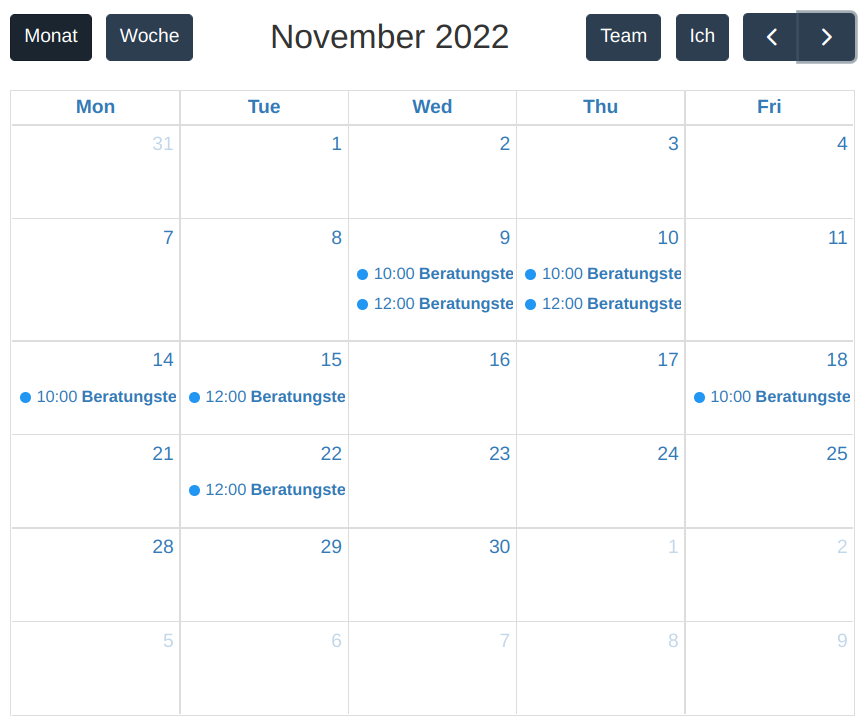
\includegraphics[width=0.9\textwidth]{screen_bremen_month_view.png}
\end{figure}

Dieses neue Ansicht ermöglicht auf den ersten Blick zu sehen, zu welcher
Uhrzeit die Termine stattfinden und einzelne Termine aus der Monatsübersicht
direkt anzuklicken. Allerdings bietet diese Ansicht keine Möglichkeit, Tage je
nach freien Plätzen rot oder grün darzustellen. Dies ist jedoch ein wichtiges
Feature für die zweistufige Terminvergabe an der zentralen Studienberatung der
Universität Kassel. An dieser Stelle braucht es eine Idee um den Hilfskräften
der Erstinformation auf den ersten Blick anzuzeigen, ob sie an diesem Tag noch
freie Terminslots vergeben können.

\paragraph{Suche nach Teilnehmern}
Manchmal kommt es vor, dass Ratsuchende, die bereits einen Beratungstermin
vereinbart haben, nochmals in Kontakt mit der Erstinformation treten, um
weitere Fragen zum Termin zu stellen. Auch kommt es vor, dass das genaue Datum
oder die Uhrzeit vergessen wurden. In diesem Fall sollen die Hilfskräfte der
Erstinformation möglichst schnell Auskunft über die angefragten Details geben
können. Hierfür immer alle vergebenen Beratungstermine manuell durchzulesen,
ist zeitlich ein großer Aufwand. Es braucht also ein Feature, sodass die
Mitarbeitenden der Erstinformationen direkt nach Terminen und weiteren
organisatorischen Daten dieser Termine suchen können. Wenn Ratsuchende
beispielsweise am Telefon ihren Namen nennen, werden sie manchmal nicht
einwandfrei verstanden. Ein Suche nach Teilnehmernamen der Termine sollte also
auch funktionieren, wenn der Name nicht exakt in der gleichen Schreibweise
eingegeben wird, wie er im Datensatz des Beratungstermins in der Datenbank
hinterlegt ist.

\paragraph{Telefonnummer Anzeige ("Silbentrennung")}
In der Regel wird bei einer Terminvergabe die Telefonnummer der ratsuchenden
Person erfasst. Der zuständige Studienberatende kann den Datensatz bei Bedarf
aufrufen und diese Telefonnummer einsehen. Dies passiert in der Regel, wenn der
Berater vor einem Beratungstermin nochmals telefonisch Details mit der
ratsuchenden Person abklären möchte. Der Berater wählt also die angezeigt
Telefonnummer in seinem Telefon. Während des Interviews im Kontext zeigt sich,
dass die Eingabe längerer Telefonnummern manchmal Fehler mit sich bringt, da
Ziffern vertauscht oder vergessen werden. Den Beratenden wäre hier eine
wertvolle Hilfe an die Hand gegeben, wenn eine Darstellung langer
Telefonnummern möglich wäre, die ein direktes und intuitives eintippen in die
Telefontastatur erleichtern.

\subsubsection{Gestaltungslösungen entwickeln}

\paragraph{Einleitung Gestaltungslösungen}
Nachdem nun die Problematiken und Herausforderungen des neuen Softwaremoduls
verdeutlicht wurden, sollen im nächsten Schritt konkrete Ideen entwickelt
werden, wie die erkannten Problematiken und Anforderungen in der Praxis
umgesetzt werden können. Alan Dix betitelt diese Phase in "Human Computer
Interaction" als "Requirements specification" und betont, dass der Fokus in
diesem Schritt darauf liegt, die notwendigen Funktionalitäten und Features der
Software grob zu beschreiben. Von besonderer Bedeutung in diesem Schritt des
Designzyklus sind Zusammenhänge und Abhängigkeiten zwischen einzelnen
Komponenten. Exakte Implementierungsdetails hingegen sind in dieser Phase noch
nicht von großer Bedeutung und sollten erst im nächste Schritt genauer
betrachtet werden.

\paragraph{Methode der Erarbeitung}
Durch die Auswertung des Interviews im Kontext sind Nutzungsanforderungen an
das neue Modul zur Terminvereinbarung entstanden. Um diese lose formulierten
Nutzungsanforderungen später implementieren zu können, werden sie in diesem
Schritt weiter konkretisiert. Es sollen erste Ideen entstehen, wie die
Bedürfnisse der Nutzenden durch einzelne Komponenten der Software umgesetzt
werden können. In diesem Fall wird mit Skizzen der einzelnen Views und
Formulare gearbeitet. Für jedes Szenario, dass Nutzende beim späteren Verwenden
der Software durchlaufen, wird eine digital gezeichnete Skizze erstellt.
Hierbei werden bereits wichtige Elemente wie Buttons, Formularfelder und
Hinweisboxen skizziert. Durch Markierungen und Notizen an der Skizze werden die
Funktionen dieser Elemente definiert.

\paragraph{Kompakte Ansicht Kalender (mit Farben)}

Die Übersicht aller Termine eines Monats ist die Ansicht, die Nutzende beim
Aufruf der Software als erstes sehen. Den größten Raum nimmt die tabellarische
Ansicht der einzelnen Tage des Monats ein. In den einzelnen Feldern werden
Terminslots, nach Uhrzeit sortiert, aufgelistet. Neben der Uhrzeit des Termins
wird der Titel eines jeden Termins angezeigt. Die einzelnen Termine werden
farblich entweder grün oder rot eingefärbt, um auf den ersten Blick zu
kennzeichnen, ob es sich um einen freien Terminslot (grün) oder um einen
bereits vergebene Termin (rot) handelt. Wenn an einem Tag viele Zeitslots
angelegt werden, wird das Feld für diesen Tag automatisch größer, sodass alle
Termine Platz finden. Sollten an jedem Tag sehr viel Termine angelegt werden,
könnte die tabellarische Monatsansicht so lang werden, dass sie unter Umständen
nicht mehr vollständig auf den Bildschirm passt. Dies wäre unpraktisch, da dann
nicht mehr alle Termine eines Monats auf einen Blick erfasst werden könnten. In
der Phase der Evaluation sollte Diese Problematik berücksichtigt werden und
eine Abschätzung getroffen werden, wie viele Termine im praktische Einsatz
tatsächlich pro Tag angelegt werden.

\begin{figure}[h]
    \caption{Monatsübersicht der Beratungstermine mit farblichen Markierungen}
    \centering
    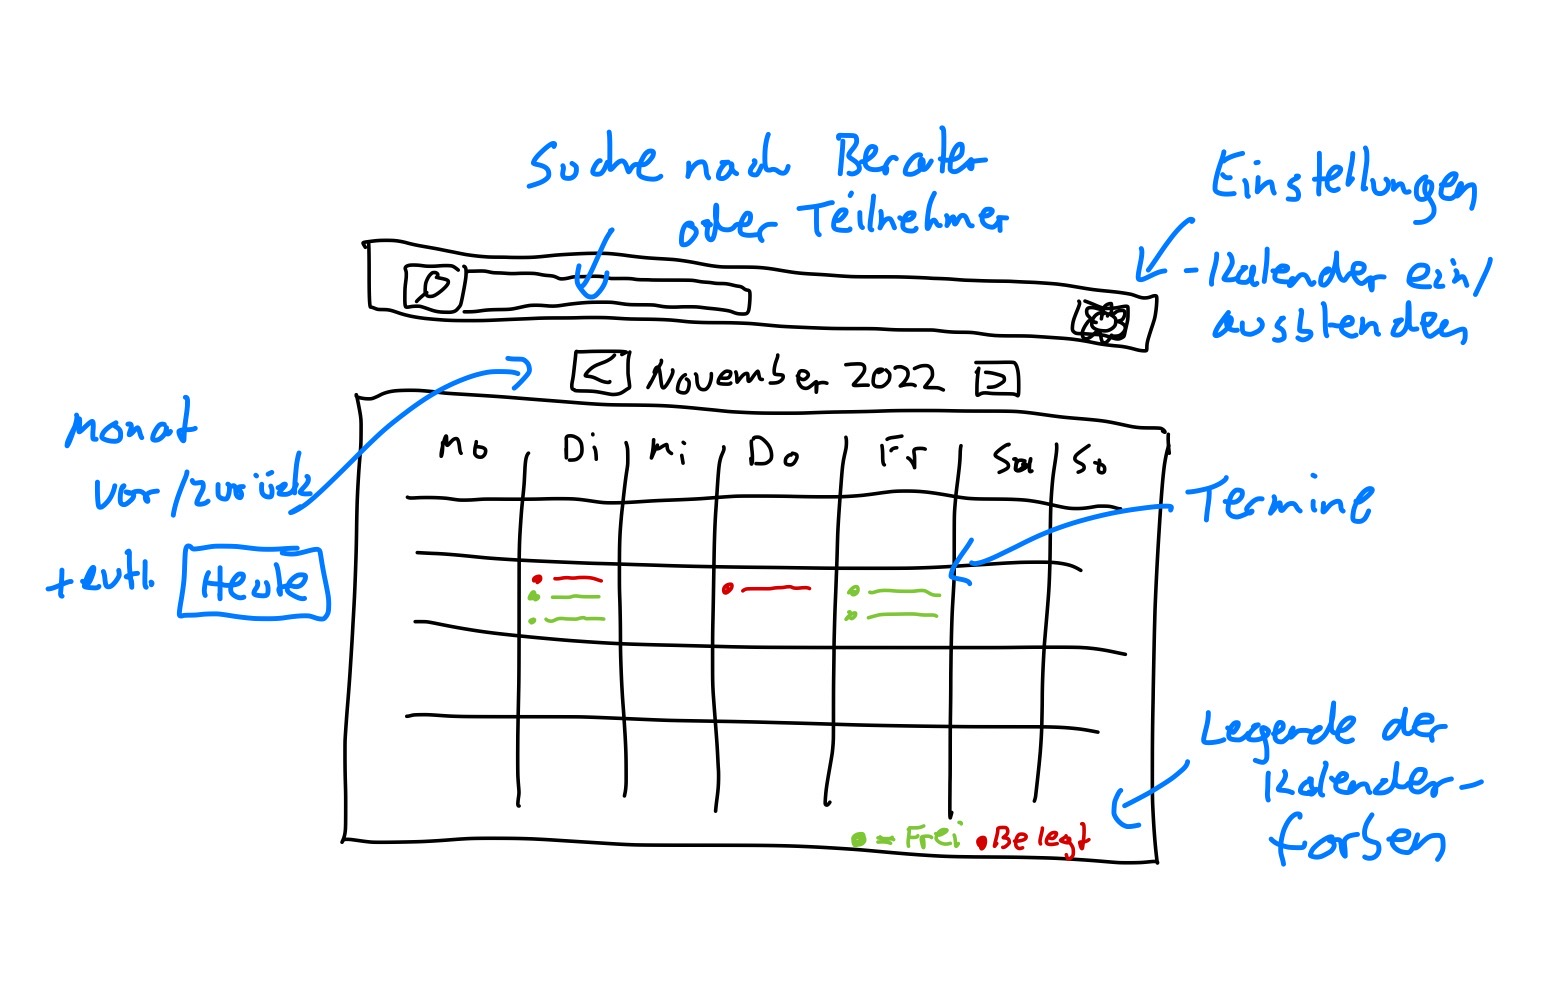
\includegraphics[width=0.9\textwidth]{doodle_month_view.jpeg}
\end{figure}

Über der tabellarischen Ansicht der Tage befindet sich eine horizontale Leiste, die den aktuell angezeigten Monat betitelt und Kontrollelemente beinhaltet um in den vorherigen bzw nächsten Monat zu wechseln. Ein Button, um nach einigem hin- und herblättern wieder den aktuelle Monat anzuzeigen, könnte in einigen Anwendungsszenarien viele Klicks ersparen. Über der Leiste mit dem Monat befindet sich eine weitere Kontrollleiste. Diese enthält einen Button um einen neuen Zeitslot anzulegen. Dieser Button sollte nur für Nutzeraccounts von Beratenden sichtbar sein. Hilfskräfte der Erstinformation sollen Zeitslots nur vergeben, aber nicht selbst anlegen können. Daneben befindet sich eine Suchleiste um schnell nach Namen von ratsuchenden Personen suchen zu können. Ganz rechts gibt es schließlich noch einen Button um weitere Einstellungen vorzunehmen. Durch einen Klick auf diesen Button mit einem Zahnrad Symbol soll ein Dropdown-Menü aufklappen, in dem Filter für die Ansicht der Termine gesetzt werden können.

\begin{figure}[h]
    \caption{Filtereinstellungen der Kalenderansicht. Das Dropdown Menü öffnet sich durch Klick auf den Zahnrad Button}
    \centering
    \includegraphics[width=0.9\textwidth]{example-image-a}
\end{figure}

In diesem Menü kann über Toggles eingestellt werden, ob nur eigene Termine oder
auch fremde Termine in der Monatsansicht dargestellt werden sollen. Mit
\textit{eigenen Terminen} sind Termine gemeint, die den eigenen Benutzeraccount
als zuständigen Beratenden hinterlegt haben. Außerdem kann ein Filter gesetzt
werden um ausschließlich freie Termine anzuzeigen. Dies kann besonders für
Hilfskräfte bei der Vergabe freier Termine relevant sein, da bereits vergeben
Zeitslots in diesem Fall irrelevante Informationen sind, die von freien
Zeitslots ablenken.

\paragraph{Suche nach Teilnehmern}

Die Suchfunktion ist ein weiterer Aspekt, dem in dieser Ausarbeitung besonderer
Aufmerksamkeit gewidmet ist. Über das Freitextfeld in der oberen Kontrollleiste
können Nutzende nach Namen von Ratsuchenden suchen, an die bereits Termine
vergeben wurden. Tippt man einige Buchstaben in das Suchfeld ein, klappt eine
Box mit Ergebnisvorschlägen unter der Suchleiste auf und schiebt den restlichen
Inhalt (die tabellarische Monatsansicht) nach unten. In diese Box werden zur
Suchanfrage passenden Termine dargestellt. Für jeden Termin wird in einer Zeile
der Titel, der Name des Ratsuchenden, der Name des Beratenden sowie Datum und
Uhrzeit aufgelistet. Neben jedem Datensatz erscheint ein Button mit einem
Augensymbol. Durch einen Klick darauf wird der entsprechende Termin in der
Detailansicht geöffnet.

\begin{figure}[h]
    \caption{Suche nach Terminen eines Ratsuchenden mit Ergebnisliste}
    \centering
    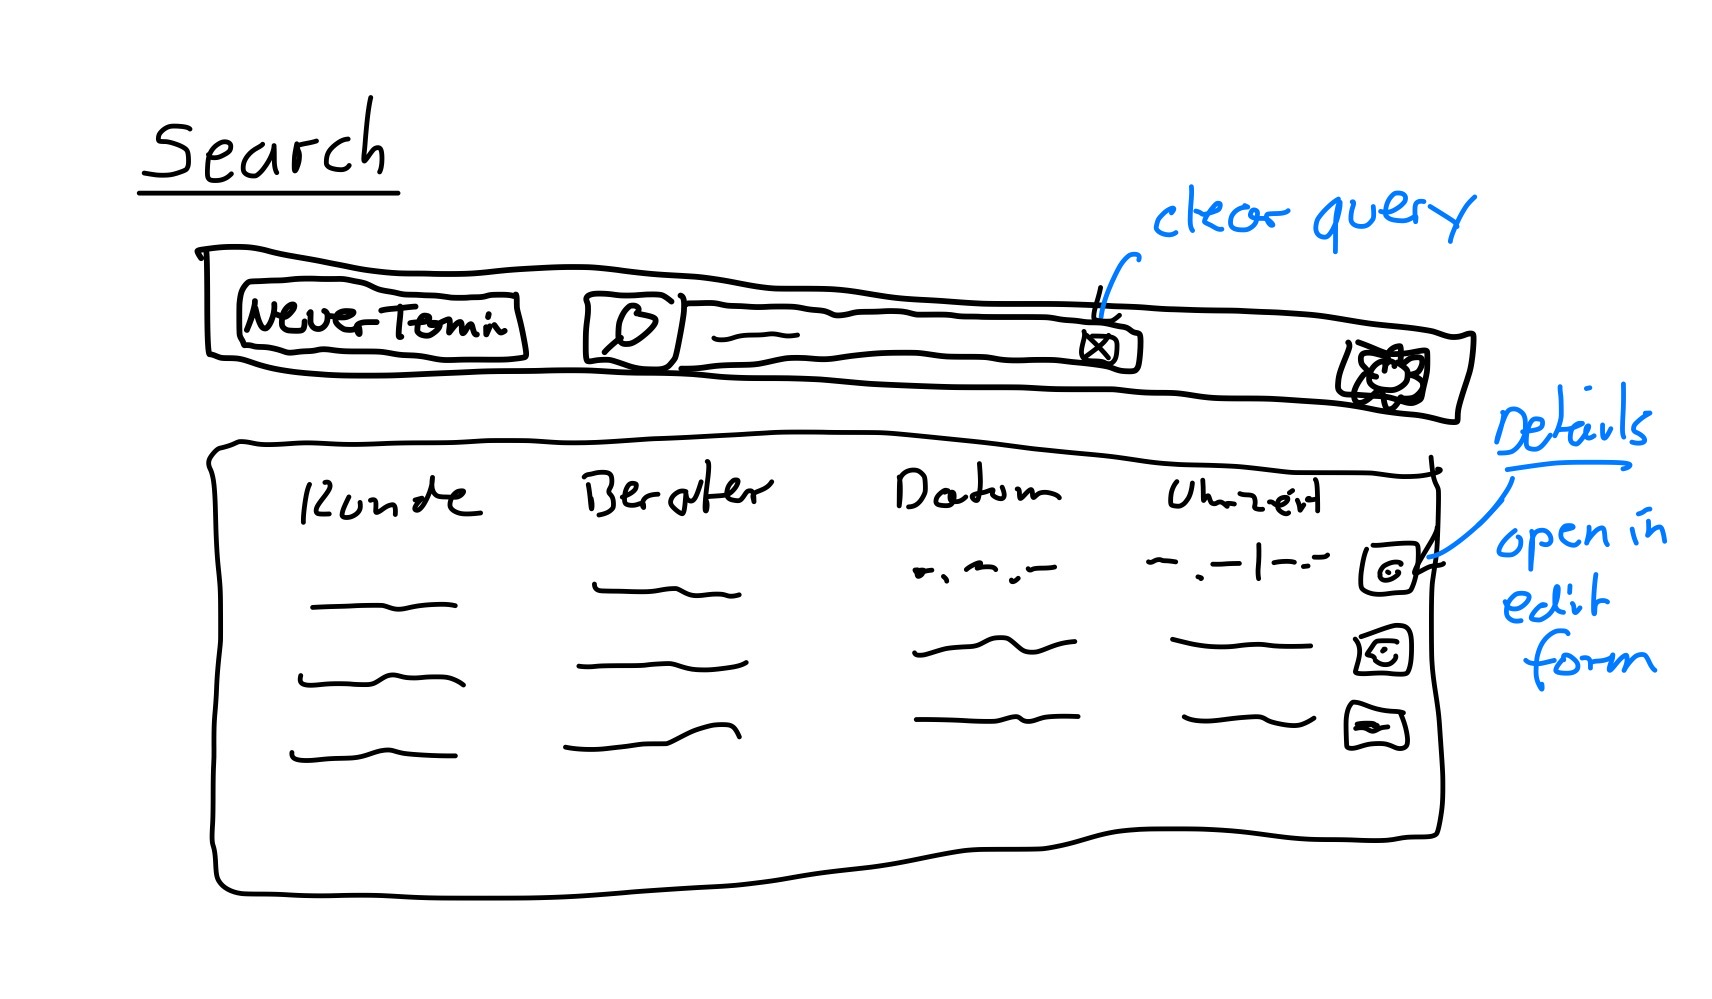
\includegraphics[width=0.9\textwidth]{doodle_search_view.jpeg}
\end{figure}

Wichtig für die Suchfunktion ist, dass passende Ergebnisse auch angezeigt
werden, wenn die Eingabe in der Suchleiste eventuell Fehler enthält oder noch
nicht vollständig ist. Durch solche automatischen Ergebnisvorschläge wird das
Suchen für die Nutzenden erleichtert und Fehlerquellen minimiert. Dadurch, dass
Nutzenden schon während dem Tippen der ersten Buchstaben ein aktives und
konstruktives Feedback erhalten, fühlt sich die Nutzung der Software
dynamischer und flüssiger an. \cite{autoCompletion} Wenn Mitarbeitende der
Erstinformation ihre Kunden am Telefon beispielsweise nicht ganz genau
verstehen, können sie mit diesen automatischen Ergebnisvorschlägen trotzdem den
passenden Termin finden. Allerdings muss bei solchen automatisiertenVorschlägen
darauf geachtet werden, dass nicht zu viele unnötige oder unpassende Vorschläge
angezeigt werden. Diese würden Nutzende von den eigentlich gesuchten
Ergebnissen ablenken und sich somit nachteilig auf die User-Experience
auswirken. \cite{autosuggModeration}

\paragraph{Telefonnummeranzeige ("Silbentrennung")}

Durch einen Klick auf den Termin in der Monatsübersicht öffnet sich die
Detailansicht des zugehörigen Termins und weitere Eigenschaften des Datensatzes
werden angezeigt. Alternativ kann ein Termin auch über die Suchfunktion
gefunden und dann über den Button mit dem Augensymbol in der Detailansicht
aufgerufen werden. In dieser Ansicht können Nutzeraccounts mit der
entsprechenden Berechtigung nochmals Details des Termins bearbeiten oder den
Termin löschen.

\begin{figure}[h]
    \caption{Detailansicht eines Termins, der bereits an eine ratsuchende Person vergeben wurde}
    \centering
    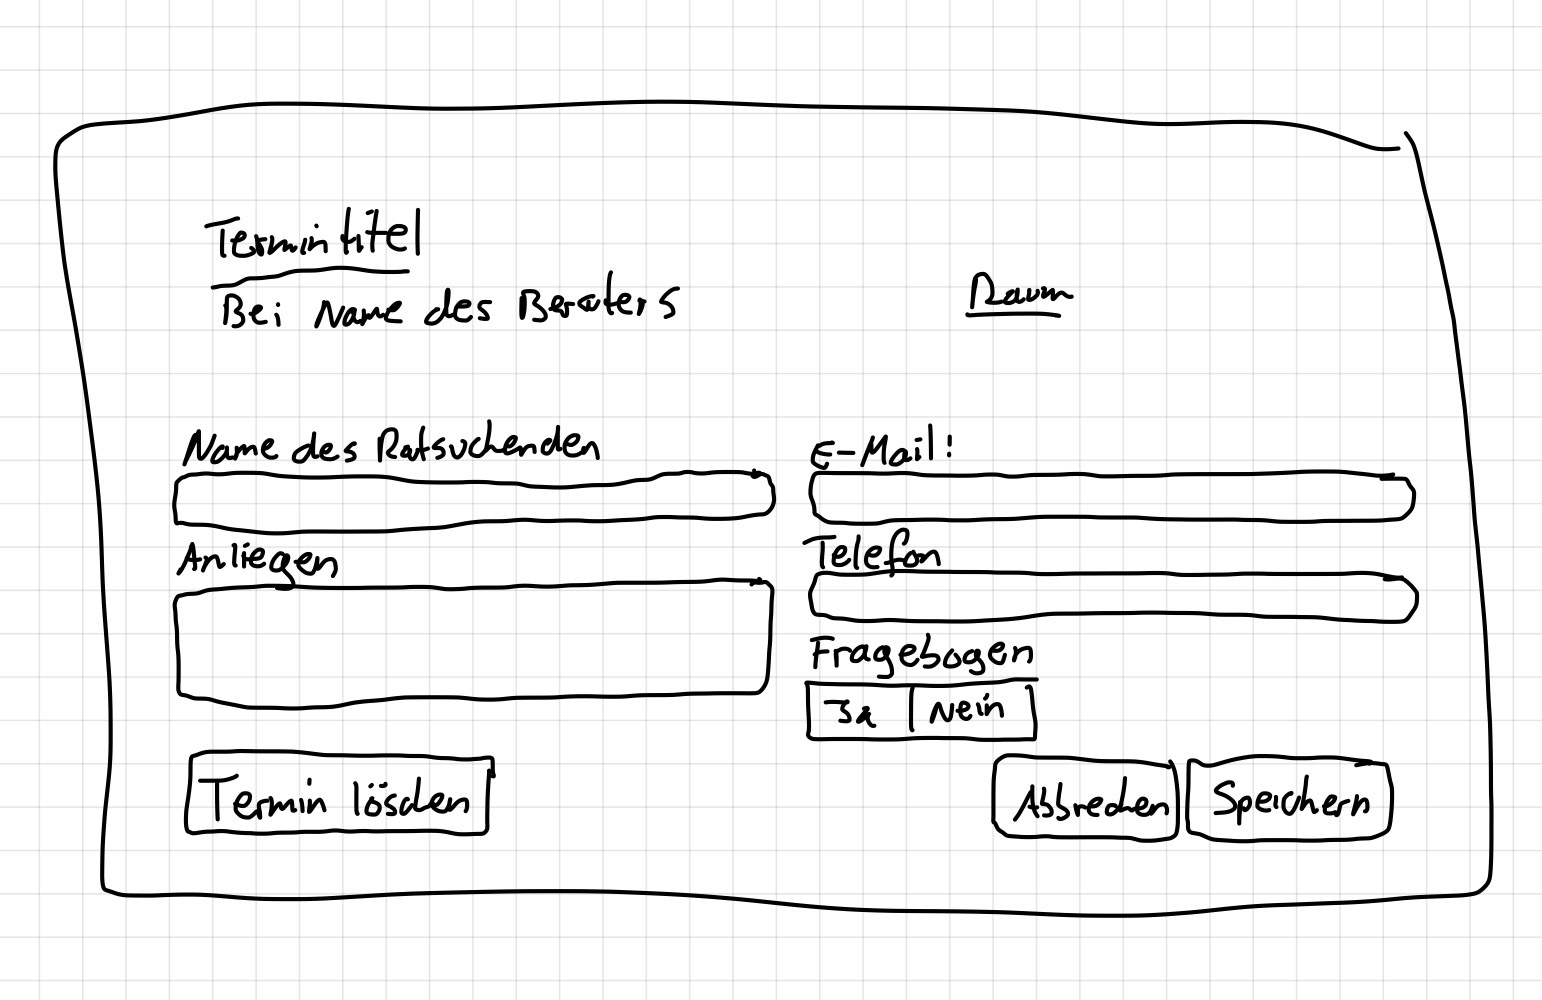
\includegraphics[width=0.9\textwidth]{doodle_client_details.jpeg}
\end{figure}

Wenn Beratende nach der Vereinbarung eines Termins nochmals auf telefonischem
Weg Absprachen oder Vorgespräche mit den Ratsuchenden erledigen möchten, können
sie die Telefonnummer der entsprechenden Person in der Detailansicht eines
Beratungstermins einsehen. Die Beobachtung des Nutzungsverhaltens während des
Interviews im Kontext hat gezeigt, dass es umständlich ist, lange
Telefonnummern zu erkennen und korrekt in die Tastatur des Telefons einzugeben.
Im Gespräch mit \ipName kam der Wunsch auf, Telefonnummern an dieser Stelle so
zu formatieren, dass sie intuitiver erfasst und abgetippt werden können. Der
Standard für das Formatieren von Telefonnummern in Deutschland wird durch DIN
5008 geregelt. Diese Norm beschäftigt sich mit Formatierungsstandards für
Briefe und Anschreiben. Hier wird das Trennen der Vorwahl vom Rest der Nummer
durch ein Leerzeichen vorgeschrieben. Weitere Formatierung, wie beispielsweise
das aufteilen der Ziffern in kleinere Blöcke wird hier nicht thematisiert.
\cite{din5008}

\begin{figure}[h]
    caption{So werden nationale Festnetz- und Mobilfunknummern nach DIN 5008 richtig geschrieben. Quelle: \cite{phoneFormatBlog}}
    \centering
    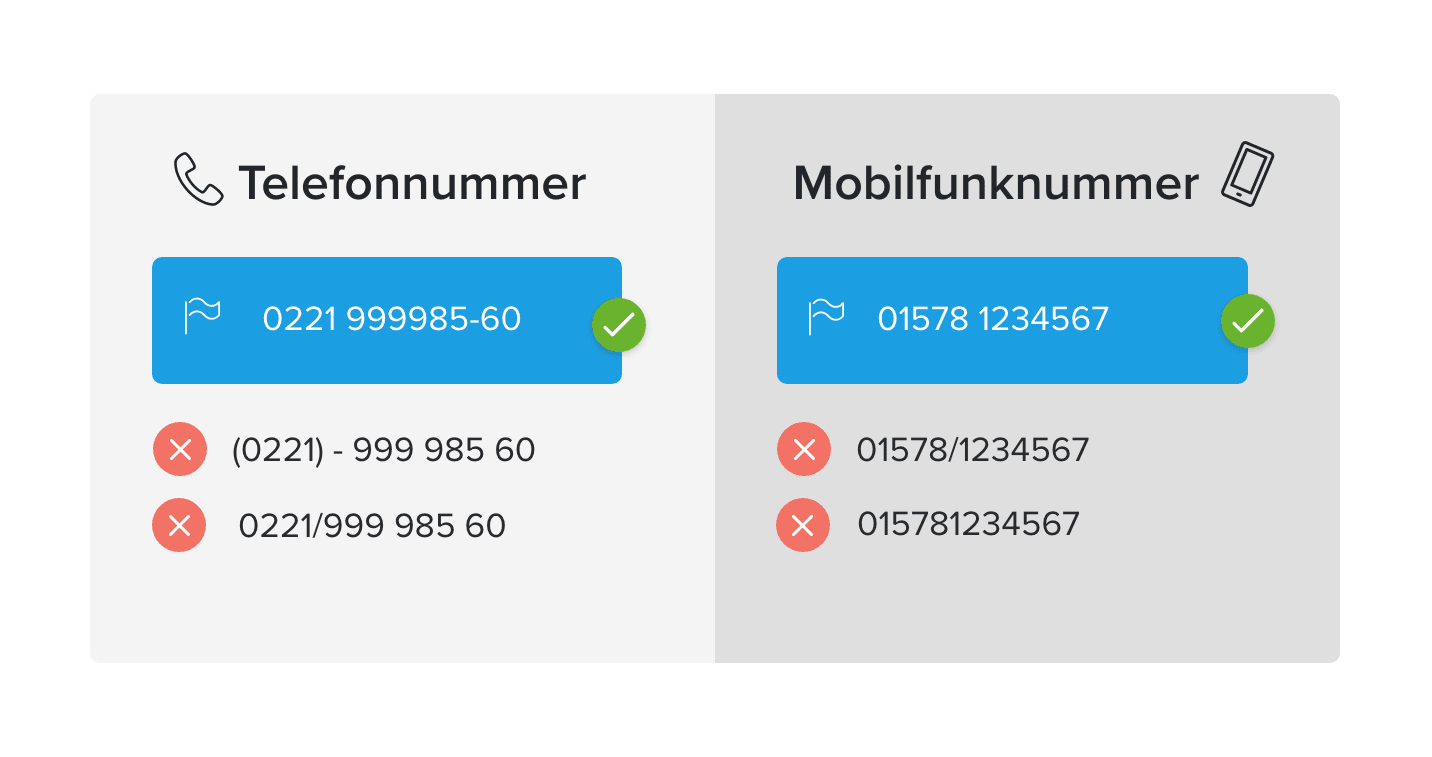
\includegraphics[width=0.9\textwidth]{grafik-telefonnummer-national.png}
\end{figure}

Wissenschaftliche Untersuchungen zeigen, dass das Eingeben und Ablesen von
Telefonnummern in Interaktion mit den entsprechenden Maschinen ein relevantes
Details ist. Dieser Prozess sollte durch die technischen Systeme möglichst
intuitiv und nutzerfreundlich gestaltet werden. \cite{humCompPhoneNumbers}.
Eine Unterteilung der Ziffern in kleinere Blöcke, von beispielsweise vier
Ziffern pro Block, erhört die Lesbarkeit deutlich und ermöglicht es dem
menschlichen Gehirn einen Ziffernblock in einem Blick direkt zu erfassen und
auf die Telefontastatur zu übertragen. \cite{phoneFormatBlog}
\cite{numberRecognition} \cite{numberRepres}

\subsection{Implementierung}
\subsubsection{Beschreibung des Prozesses}

\paragraph{Überleitung}
Im vorherigen Schritt wurden konkrete Nutzungsanforderungen herausgearbeitet
und Ideen für passende Gestaltungslösungen formuliert. Nun soll das folgende
Unterkapitel sich mit der praktischen Umsetzung der Anforderungen beschäftigen.
Dieser Prozess entspricht dem dritten Schritt \glqq{}Gestaltungslösungen
entwickeln, die die Nutzungsanforderungen erfüllen\grqq{} des Designzyklus im
Human Centered Design nach ISO 9241\cite{iso9241}.

\paragraph{Kundenwünsche und Technische Machbarkeit}
Auch wenn im Human Centered Design immer die Nutzenden und nicht das technische
System im Fokus stehen sollte,kommt man nicht drumherum die technischen Details
genauer zu betrachten. Dadurch ist es ganz besonders wichtig in dieser Phase
die Bedürfnisse und Erwartungen der Nutzenden nicht aus den Augen zu verlieren.
Eine klare und intuitive Schnittstelle für die Nutzenden sollte in diesem
Prozess eine höhere Priorität einnehmen als eine Lösung, die technisch am
einfachsten umzusetzen ist. K. Holtzblatt verwendet hier den Begriff
\textbf{Kohärenz} und meint damit, das sich ein System für den Nutzer so
zusammenhängend und natürlich wie möglich anfühlen soll: \glqq{}The challenge
is to keep the system work model coherent, so that it supports the users and
fits with their expectations while extending and transforming their work
practice as prescribed by the vision.\grqq{}\cite{contextualDesign}.
Gleichzeitig müssen alle Lösungsansätze natürlich auch tatsächlich programmiert
werden können. Hierbei kann nicht ignoriert werden, dass viele externe Faktoren
die Machbarkeit bestimmter Lösungskonzepte in der Praxis einschränken. G.A. Boy
erwähnt in \textit{The Handbook of Human-Machine Interaction} einige dieser
Faktoren: \glqq{}Design work is often constrained by various external factors
in the development organization and the marketplace (policies, standards,
competitive products, past and planned products, schedules, resource
budgets).\grqq\cite{HMI-HCD} So ermöglichen verwendete Programmiersprachen,
eingesetzte Frameworks und bereits existierende Softwareteile es, bestimmte
Konzepte sehr elegant umzusetzen. Andere Gestaltungsideen sind, beschränkt
durch äußere Faktoren, unter Umständen gar nicht realisierbar.\cite{HMI-HCD}

\paragraph{Überleitung konkreter Anwendungsfall Stubegru}
In dem konkreten Fall des erarbeiteten Moduls zur Terminvergabe für die
Studienberatung ist hier ein wichtiger Gesichtspunkt, dass es sich um ein Modul
innerhalb eines bereits bestehenden Softwarepakets handelt. Tech-Stack,
Programmiersprache und Schnittstellen zu anderen Modulen sind hier bereits
vorgeben und können nicht allein durch die Wünsche der Nutzenden geformt
werden.

\paragraph{Techstack Stubegru}
Im Folgenden sollen nun die technischen Gegebenheiten und Grundlagen der
Software \textbf{Stubegru} vorgestellt werden. Das neue System zur
Terminvereinbarung muss sich als Modul in das Softwarepaket Stubegru einbinden
lassen und somit einige Standards und Schnittstellen der Software zur Verfügung
implementieren.

Die Software Stubegru ist webbasiert und wird über einen Browser aufgerufen.
Dementsprechend sind die verwendeten Technologien im Frontend Html, Css und
Javascript. Die Kommunikation mit dem Backend wird durch asynchrone
Http-Requests umgesetzt, die durch Javascript Methoden initiiert werden. Das
Backend besteht aus vielen einzelnen Php Dateien, welche die per Http
übermittelten Daten auslesen und aufarbeiten. Als Datenbank kommt eine
relationale mySQL Datenbank zum Einsatz, die von den Php Skripten über
Php-Database-Objects (PDO) angesprochen wird. Die abgerufenen Daten der Php
Skripte werden, als JSON codiert zurück an das Frontend geschickt und dort von
Javascript Methoden weiterverarbeitet. Mithilfe der Javascript Library jQuery
werden die entsprechende Element im Document Object Model (DOM) angepasst und
somit für den Nutzenden grafisch dargestellt. Das Softwarepaket Stubegru ist
grundlegend modular aufgebaut, sodass für jede Funktionalität oder jeden
Prozess ein eigenes Modul programmiert wird, das genau diese Aufgabe übernimmt.
Jedes Modul besteht aus den entsprechenden Anzeigeelementen, die in einer Html
Datei formuliert werden. Des weiteren grafische Designregeln, die als CSS Datei
angelegt werden und der eigentlichen Logik, die in Javascript implementiert
werden muss. Im Modul zur Terminvereinbarung kommt zusätzlich die Javascript
Library \textbf{fullcalendar} zum Einsatz. Diese bietet eine einfache
Schnittstelle um Termindaten in einer monatlichen Übersicht darzustellen und
bietet dem Nutzenden standardisierte Kontrollelemente zum Interagieren mit der
Kalenderansicht. Funktionalitäten wie das Rendern einer Monatsübersicht, oder
das Wechseln zwischen den einzelnen Monaten sind über diese Bibliothek bereits
abgedeckt und müssen nicht eigenständig implementiert werden. Gleichzeitig
schränkt die Verwendung dieser Bibliothek die Möglichkeiten in der Darstellung
der Termine auch ein, sodass lediglich die angebotenen Ansichten
(Monatsansicht, Wochenansicht, Tagesansicht, Terminliste) eingesetzt werden
können.

\subsubsection{Nutzungsanforderungen formalisieren | Sequenzdiagramme}
\label{subsection:sequenceDiagrams}

\paragraph{Einführung Sequenzdiagramme}
Um die erarbeiteten Nutzungsanforderungen in praktische Programmierung
umzusetzen wurden zunächst Sequenzdiagramme erstellt. Diese Diagramme werden
jeweils für einen zusammenhängenden Workflow gezeichnet und skizzieren alle
kleinere Teilschritte, die in diesem Workflow nacheinander abgearbeitet werden
sollen. Ziel eines Sequenzdiagramms ist es, die einzelnen Aktivitäten, die ein
Nutzender beim Verwenden der Software durchläuft,
darzustellen.\cite{holtzblattCDEvolved} An solchen Diagrammen können auch die
Zusammenhänge dieser Aktivitäten untereinander abgelesen werden. Karen L.
McGraw verweist in \textit{User-centered Requirements} darauf, dass diese Art
von Diagrammen sehr hilfreich sein können, um primäre Workflows und
zusammenhängende Prozesse zu identifizieren\cite{sequenceDiagrams}. Ian
Alexander führt in \textit{Scenarios, Stories, Use Cases} ganz ähnliche
Diagramm ein, die er Scenario Process Models nennt. Auch hier geht es darum ein
Abbild der Teilprozesse zu schaffen, die ein Nutzender beim Verwenden eine
Software durchläuft. I. Alexander nennt als weiteren Vorteil dieser Diagramme,
das noch unklare oder fehlende Daten innerhalb eines Workflows schnell zu
erkennen sind. Über eingehende und ausgehende Pfeile kann an den
Sequenzdiagrammen abgelesen werden durch welche Aktionen der jeweilige Workflow
angestoßen wird, beziehungsweise welche anderen Workflows durch
Nutzerinteraktionen angestoßen werden können. Teile einzelner Elemente der
grafischen Oberfläche werden zkizzenhaft dargestellt, um einen intuitiven
Eindruck festzuhalten, wie die Nutzenden durch diesen Workflow navigieren und
welche Steuerelemente sie auf dem Bildschirm verwenden können. Durch farbige
Anmerkungen an einzelnen Elementen oder Arbeitsschritten wird auf bestimmte
Details hingewiesen, die bei der Implementierung zu beachten sind. So kann
beispielsweise angemerkt werden, dass nach einem Klick auf einen Button, ein
Popup mit einer Bestätigungsaufforderung angezeigt werden soll. Die
Sequenzdiagramme sind bewusst formlos gehalten und nur grob skizziert. Dies
spiegelt die schnelle und intuitive Erstellung dieser Diagramme wieder. Es geht
noch nicht darum den Prozess in einer sehr strukturierten Darstellungsform
aufzuzeichnen, die man direkt in Code übersetzen könnte. Vielmehr soll intuitiv
und spontan festgehalten werden, welche Schritte ein Nutzender durchlaufen
könnte, wenn er jenen Workflow anstößt.

\paragraph{Beispiel Sequenzdiagramm [Vergebenen Termin aufrufen]}
Beispielhaft für den Entstehungsprozess dieser Sequenzdiagramme wird im
Folgenden ein Diagramm gezeigt und näher erläutert. Dieses Diagramm beschreibt
den Workflow wenn ein Nutzender die Detailansicht eines bereits vergebenen
Termins aufruft.

\begin{figure}[h]
    \caption{Sequenzdiagramm, Laden der Detailansicht für einen vergebenen Termin}
    \centering
    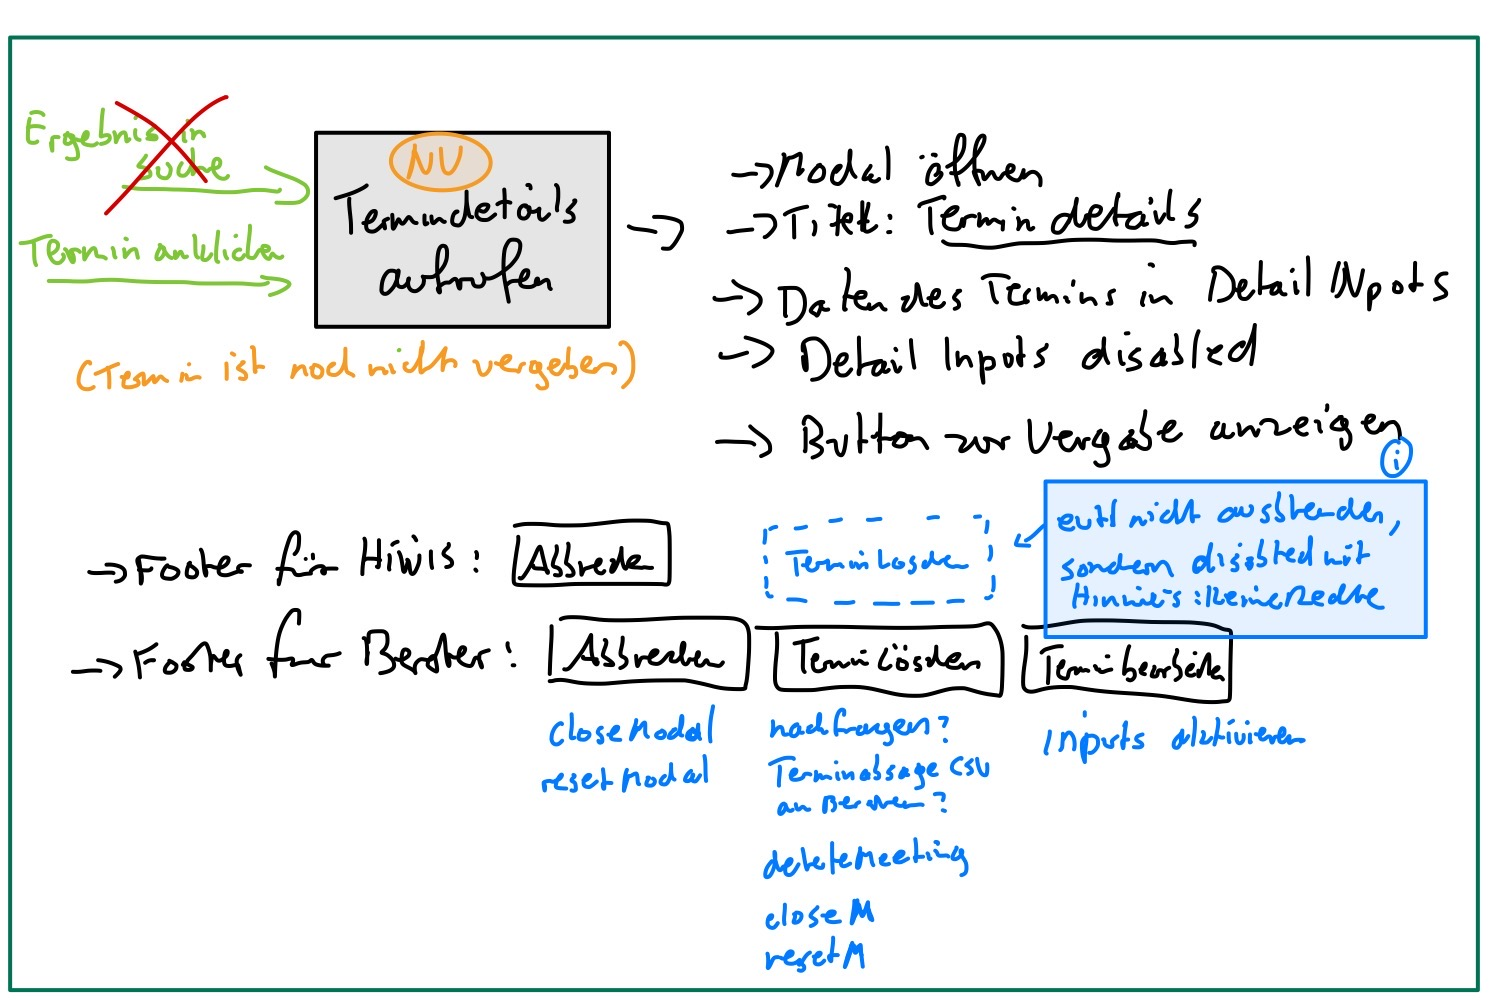
\includegraphics[width=0.9\textwidth]{flow_termin_aufrufen_unvergeben.jpeg}
\end{figure}

Die grünen Pfeile links oben beschrieben, auf welchem Weg Nutzenden diesen
Workflow anstoßen können. Die Detailansicht eines vergebenen Termins kann in
diesem Fall auf zwei verschiedenen Wegen geöffnet werden. Entweder klickt ein
Nutzender auf einen Termin in der Monatsübersicht oder er klickt auf ein
Suchergebnis in der Ergebnisliste der Suche nach Teilnehmenden. Im rechten
oberen Teil des Diagramms wird stichpunktartig festgehalten, welche
Teilschritte notwendig sind um die Termindetails sinnvoll darstellen zu können:
Zunächst muss das Modal\todo{Modal im Glossar} über dem bestehenden
Bildschirminhalt eingeblendet werden. Im nächsten Schritt muss der Titel des
Modals angepasst werden. Der Standardtitel \textit{Termin erstellen} macht in
diesem Kontext keinen Sinn, da der Termin bereits existiert. Daher wird der
Titel des Modals in diesem Fall auf \textit{Termindetails} geändert. Im
weiteren Verlauf müssen die Daten des Termins (Datum, Uhrzeit, Titel) in die
entsprechenden Input Felder geladen werden. Diese Input Felder sollen als
\textit{disabled} dargestellt werden. Das bedeutet, dass man den eingetragenen
Inhalt lesen, ihn jedoch nicht bearbeiten kann. Ein bereits an einen Kunden
vergebener Termin kann nicht bearbeitet werden, solange der Datensatz des
Kunden nicht entfernt wurde. So soll vermieden werden, dass beispielsweise das
Datum des Beratungstermins nachträglich geändert wird, ohne dass der Kunde
darüber informiert wird. Hier wird den Nutzenden also bewusst die
Funktionalität des nachträglichen Änderns verboten, um keine Missverständnisse
mit der Kundschaft aufkommen zu lassen. Sollte tatsächlich einmal das Datum
eines Beratungstermins verändert werden, muss der Kundendatensatz zunächst
entfernt und dann, nach dem Anpassen des Datums neu hinzugefügt werden, Dies
hat den Vorteil, dass die entsprechenden Informationsmails (Terminabsage, Neue
Terminbestätigung) korrekt an den Kunden und den Beratenden gesendet werden und
somit für beide Parteien nachvollziehbar ist, an welchem Datum der Termin nun
tatsächlich stattfinden soll.

\begin{figure}[h]
    \caption{Verschiedene Bereiche des Modals mit Kontrollelementen}
    \centering
    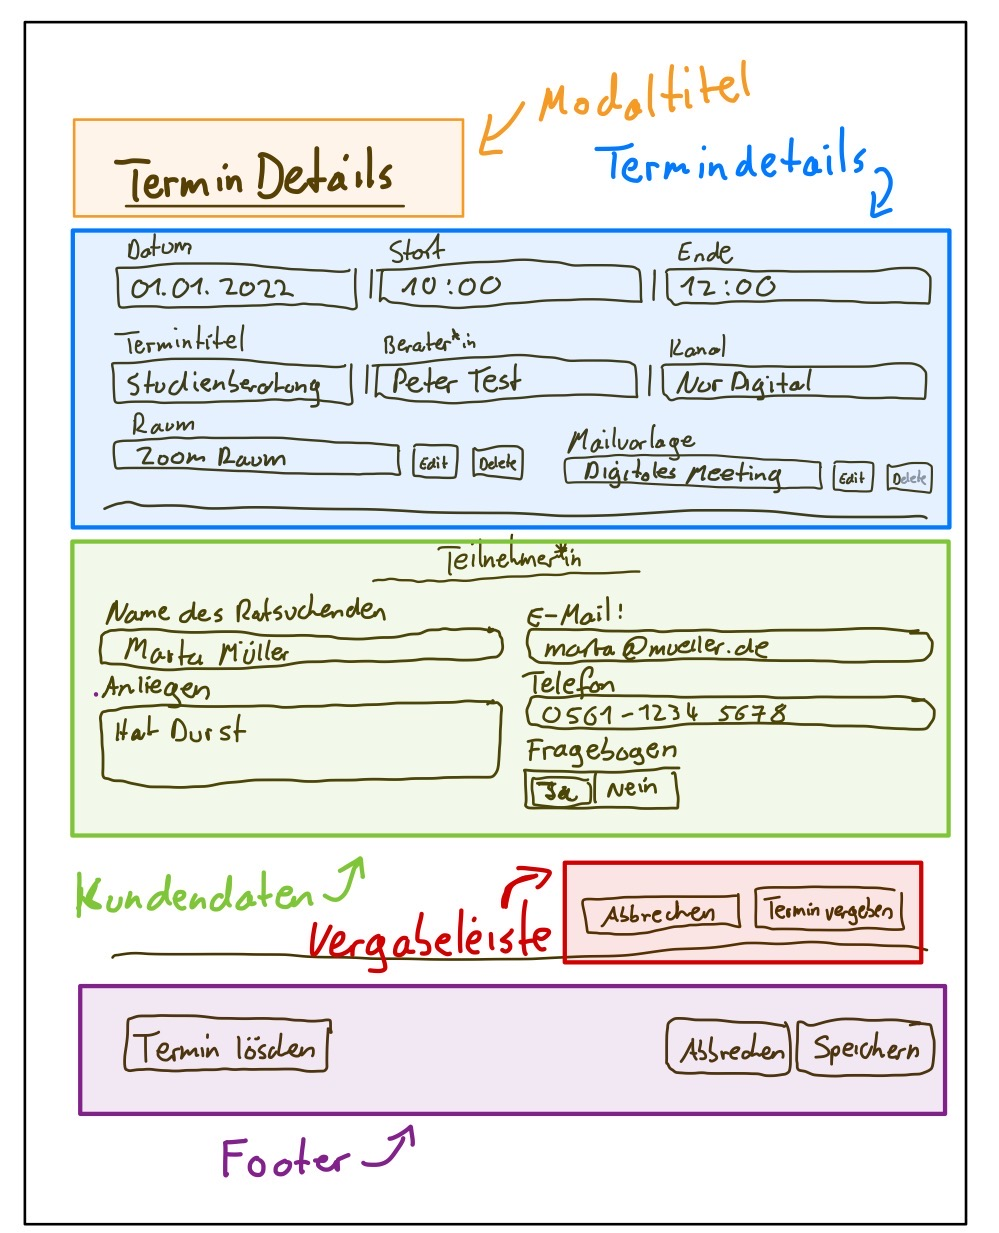
\includegraphics[width=0.9\textwidth]{doodle_modal_overview.jpeg}
\end{figure}

Im unteren Teil des Diagramms wird durch kleine Skizzen festgehalten, welche
Kontrollelemente den Nutzenden im Workflow zur Verfügung stehen. Die
Textit{Vergabestelle} bezeichnet den Bereich, indem Buttons zum Interagieren
mit den Kundendaten dargestellt werden. In diesem Fall ist lediglich der Button
\textit{Kundendaten löschen} sichtbar. Ein nachträgliches Bearbeiten der
Kundendaten soll nicht möglich sein, da auch hier inkonsistente Status beim
Versand der Mails an den Kunden entstehen könnten. Wird beispielsweise die
Mailadresse des Kunden geändert, nachdem er für den Versand eines
Feedback-Fragebogens eingetragen wurde, kann der Link für den Fragebogen nicht
mehr an die korrekte Adresse verschickt werden. Diese Problematik wird im
Diagramm grafisch durch die orangene Infobox am rechten Rand verdeutlicht.
Schlussendlich wird im Diagramm dargestellt welche Buttons in der Fußleiste des
Modals angezeigt werden sollen. Hier soll lediglich der Button
\textit{Abbrechen} aktiv sein. Über diesen Button wird das Modal ohne Übernahme
von Änderungen geschlossen und ein anderer Termin kann aufgerufen werden. Die
Buttons zum Speichern und Löschen des Termins sollten nicht angeklickt werden
können. Wie bereits erwähnt, soll ein Ändern oder Löschen der Termindaten nur
möglich sein, wenn die verknüpften Kundendaten entfernt wurden. Die Buttons
sollen jedoch nicht vollkommen unsichtbar sein, sondern lediglich ausgegraut
dargestellt werden. Die blaue Box im Diagramm ergänzt, das bei einem
Mouse-Hover über diese ausgegrauten Buttons ein Hinweis angezeigt werden soll.
Dass die Buttons nicht vollständig ausgeblendet werden, sondern stattdessen
deaktiviert mit einem Hinweis dargestellt werden, soll dazu führen, dass
Nutzende eine einheitliche Benutzeroberfläche vorfinden und bei dem Versuch mit
den deaktivierten Buttons zu interagieren, automatisch darauf hingewiesen
werden, welche Schritte notwendig sind, um die gewünschte Funktion nutzen zu
können. Dieser Ansatz soll dazu beitragen, dass auch unerfahrene Nutzende
schnell und intuitiv verstehen, wie eine Interaktion mit dem System gedacht
ist.

Im Anhang \todo{Referenz einfügen} finden sich weitere drei Sequenzdiagramme
die folgende Prozesse beschreiben: \textit{Vergebenen Termin aufrufen},
\textit{Neuen Termin erstellen} und \textit{Termin an Kunden
    vergeben}\todo{Diagramme einfügen}.

\subsubsection{Technische Umsetzung}

\paragraph{Überleitung Technische Details}
Im folgenden Abschnitt soll der Fokus nun auf die technischen Details der
Implementierung gelegt werden. Wesentliche Fragestellungen sind hier: Wie
werden die Nutzungsanforderung in der Praxis umgesetzt? Welche Designpattern
und Softwarekonzepte werden verwendet? Wie werden Schnittstellen zwischen
Frontend und Backend gestaltet? Und über welche Protokolle werden Daten
ausgetauscht? Wichtig ist es, an dieser Stelle wieder im Blick zu behalten,
dass es sich um eine Modul in einer bereits bestehenden Software handelt. Somit
sollten bereits existierende Konzepte und Schnittstellen nach Möglichkeit
wieder verwendet werden. Durch das Aufgreifen bestehender Lösungsstrategien und
Entwurfsmuster wir das gesamte Softwarepaket einheitlich strukturiert und ist
somit leichter zu warten. Gleichzeitig müssen einige Funktionen nicht von Grund
auf neu implementiert werden, somit kann Zeit und Arbeit in diesem Prozess
erspart werden.\cite{wiederverwSoftware} Im Folgenden werden einige
Designentscheidung, Grafiken und Codeschnipsel präsentiert um einen groben
Einblick in die technische Umsetzung zu erlauben. Der vollständige Sourcecode,
sowie alle Commits zur Programmierung des Moduls sind im entsprechenden GitHub
Repository einzusehen.\cite{stubegruRepo}

\paragraph{Datenmodell}
Die eigentlichen Datenmodelle mit denen in dem Modul zur Terminvereinbarung
gearbeitet wird sind relativ simpel gehalten. Es gibt drei relevante Typen von
Datensätzen: Termine, Mailtemplates und Beratungsräume. Die Datensätze, die
einen Termin beschreiben, enthalten außerdem auch Informationen über den
Ratsuchenden, der diesen Termin gebucht hat. Diese Datensätze werden im
Folgenden als Meeting bezeichnet und sollen anhand eines UML Diagramms
detailliert veranschaulicht werden.\todo{UML erklären?}

\begin{figure}[h]
    \caption{UML Diagramm der Klasse Meeting. Stellt alle Methoden und Eigenschaften eines Objektes dar, das einen Termin repräsentiert}
    \centering
    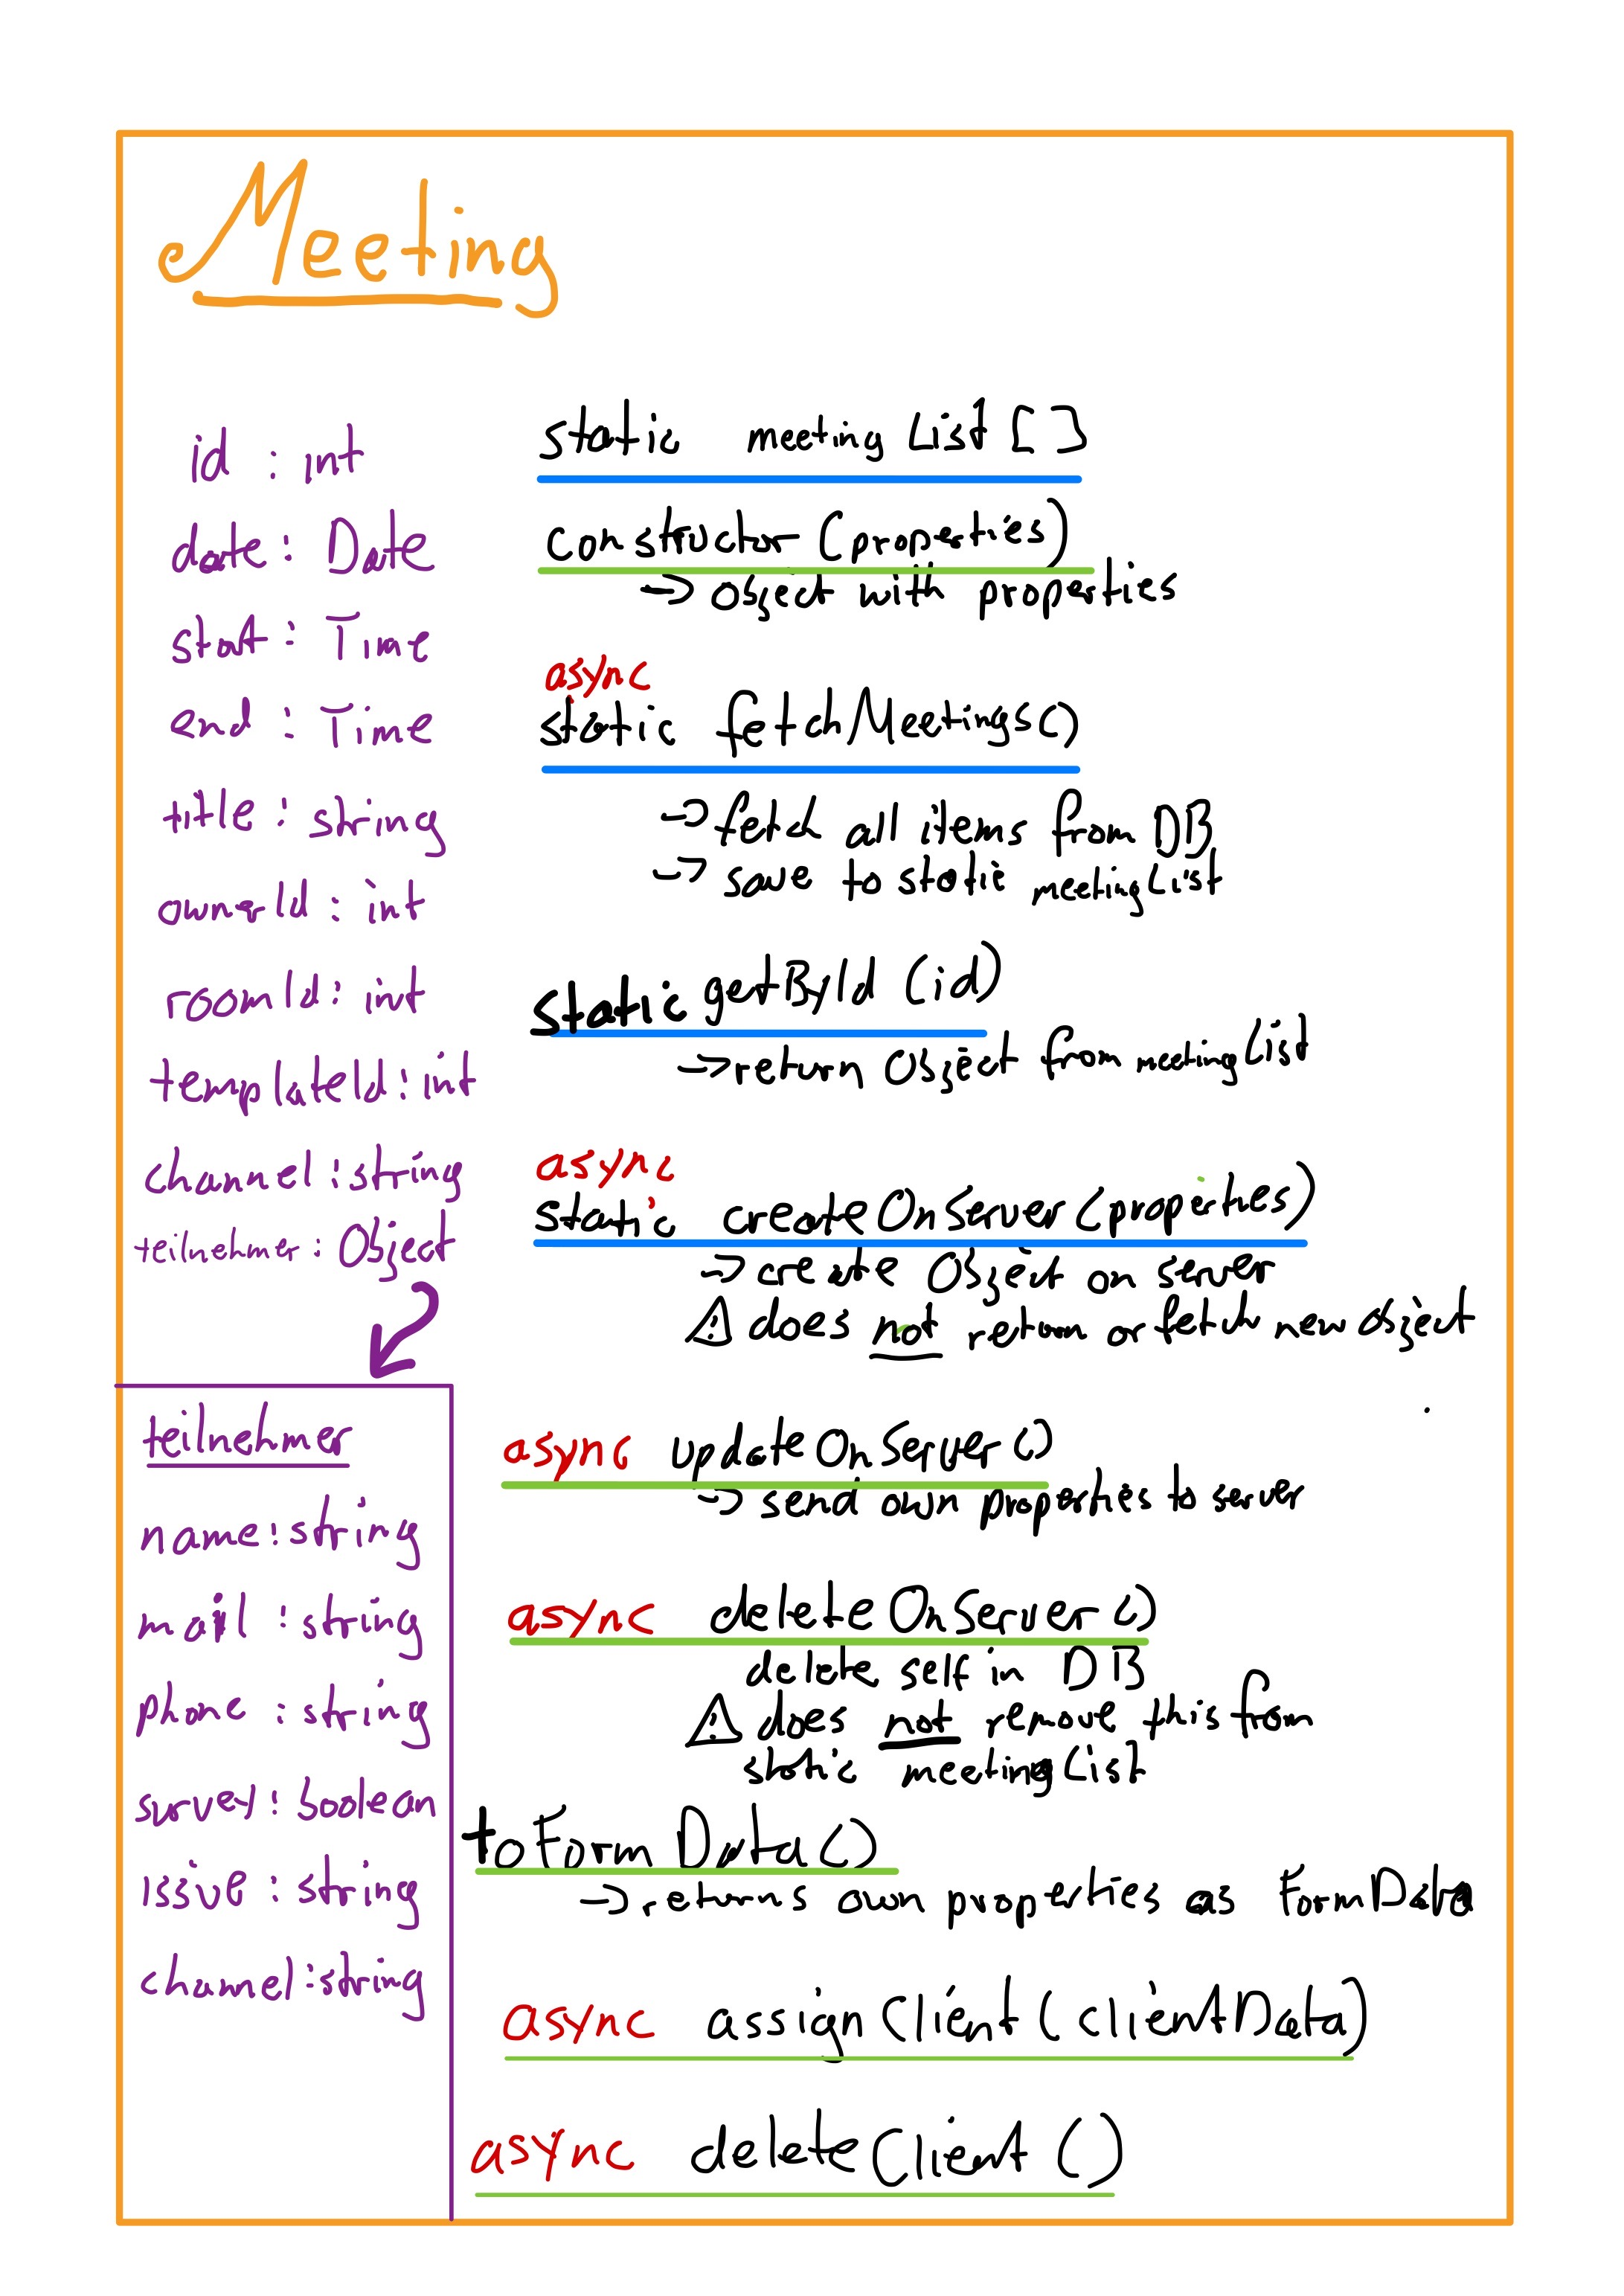
\includegraphics[width=0.9\textwidth]{uml_meeting.jpeg}
\end{figure}

Die Klasse Meeting stellt zunächst einige statische Eigenschaften und Methoden
zur Verfügung. Das Array \textit{meetingList} enthält zur Laufzeit alle aktuell
bekannten Meetings in einer unsortierten Liste. Durch die statische Funktion
\textit{fetchMeetings()} werden alle Datensätze aus der Datenbank geladen und
in der \textit{meetingList} gespeichert. Über die Funktion \textit{getById()}
kann ein bestimmtes Meeting aus der \textit{meetingList} angesprochen werden.
Die weiteren Funktionen dienen dazu, die Eigenschaften eines Meetings an das
Backend zu senden, um die neuen Werte in der Datenbank zu speichern oder zu
löschen. Die statische Methode\textit{createOnServer(properties)} sendet die
Daten eines neuen Meetings an den Server. Diese Methode erstellt bewusst keine
neue Instanz vom Typ Meeting, da es keinen Sinn macht ein Meeting Objekt zu
verwenden, solange der Server dieses Meeting noch gar nicht kennt. Im Anschluss
an die \textit{createOnServer(properties)} Methode sollte stets die Methode
\textit{fetchMeetings()} aufgerufen werden, um auf das neu erstellte Meeting
zugreifen zu können. Die Funktion\textit{updateServer()} wird auf einem
bestehenden Objekt vom Typ Meeting aufgerufen und sendet die aktuellen lokalen
Eigenschaften an den Server. Hierbei wird die Funktion\textit{toFormData()}
verwendet, um die Eigenschaften des Objektes in das passende Format zu bringen.
Die so aufbereiteten Daten werden über den asynchronen Aufruf der
\textit{fetchApi}\cite{fetchAPI} mit einer HTTP Request an das entsprechenden
PHP Skript auf dem Server gesendet.

\lstinputlisting[language=Java, caption=Senden von lokalen Änderungen eines Meetings an den Server]{listings/updateOnServer.js}

Über die Methode \textit{deleteOnServer()} kann ein bestehendes Meeting auf dem Server gelöscht werden. Durch einen anschließenden Aufruf von \textit{fetchMeetings()} wird das Meeting dann auch in der lokalen \textit{meetingList} gelöscht. Außerdem stellt ein Objekt vom Typ Meeting noch zwei Methoden zur Verfügung um Kundendaten zu verknüpfen beziehungsweise zu löschen. Diese Funktionen stoßen in den jeweiligen PHP Skripten auf dem Server weitere Workflows an, wie beispielsweise das Versenden einer Bestätigungsmail an die ratsuchende Person.

\lstinputlisting[language=PHP, caption=PHP Skript zum Erstellen eines neuen Meetings in der Datenbank]{listings/save_meeting.php}

\paragraph{Workflow: Vergebenen Beratungstermin aufrufen}

In Kapitel \ref{subsection:sequenceDiagrams} wurden exemplarisch alle Teilschritte erklärt, die nötig sind um einen bereits vergebenen Beratungstermin aufzurufen und in der Detailansicht darzustellen. Für jeden dieser einzelnen Schritte wurde eine entsprechende Funktion in der Klasse \textit{CalendarModal} implementiert. Die Funktion \textit{setModalVisible(isVisible)} kann beispielsweise aufgerufen werden um das Modal ein- oder auszublenden. Die Klasse \textit{CalendarController} verwendet nun all diese Funktionen und bildet so den kompletten beschriebenen Workflow Schritt für Schritt ab. Das folgende Listing beschreibt den Ablauf aller einzelnen Schritte durch den sequenziellen Aufruf der einzelnen Funktionen:

\lstinputlisting[language=Java, caption=Öffnen der Detailansicht eines vergebenen Beratungstermins]{listings/openAssignedMeeting.js}

\paragraph{Monatsansicht mit fullcalendar darstellen}

Als abschließendes Beispiel der konkreten Implementierung wird die Klasse \textit{CalendarView} vorgestellt. Diese ist für das Darstellen der Terminübersicht zuständig. An dieser Stelle wird die Javascript Bibliothek \textit{fullcalendar}\cite{fullCalendarWeb} verwendet um den Aufbau der Monatsansicht deutlich zu vereinfachen. Die Klasse \textit{CalendarView} referenziert auf eine Instanz vom Typ \textit{FullCalendar} und kann darüber die wichtigsten Funktionen zum Löschen und Hinzufügen weiterer Termine aufrufen.
Im folgenden Listing wird die Funktion \textit{addMeetings(meetingList)} gezeigt. Diese Funktion wird vom \textit{CalendarController} aufgerufen und bekommt als Parameter eine Liste von Meetings übergeben. Aus den übergebenen Objekten vom Typ \textit{Meeting} werden zunächst Objekte generiert, die alle Eigenschaften erhalten, welche die \textit{fullcalendar} Bibliothek benötigt um die Termine in der Übersicht korrekt anzeigen zu können. Die so erstellten Datensätze werden anschließend in \textbf{eigene Termine} und \textbf{fremde Termine} sortiert. Über die Funktion \textit{fullCalendar.addEventSource(eventSource)} werden die Listen mit den eigenen und den fremden Terminen hinzugefügt. Über den weiteren Parameter \textit{color} wird in diesem Fall die farbliche Darstellung der Termine in der Monatsübersicht gesteuert.

\lstinputlisting[language=Java, caption=Hinzufügen von Terminen in die Monatsübersicht von fullcalendar]{listings/addMeetings.js}
    
\subsection{Testen / User-feedback}
\subsubsection{Methode ???}
\subsubsection{Präsentation erster Ergebnisse}
\subsubsection{Feedback der Nutzenden}
\subsubsection{Ausblick auf weitere Iterationen}
\section{Reflektion und Fazit}
\paragraph{Einleitung Kapitel Fazit}

\subsection{Beschreibung der Ergebnisse}
\paragraph{Was war geplant, was wurde umgesetzt?}
\paragraph{Umsetzung von Feedback des Usertests}


\begin{figure}[H]
    \caption{Details eines vergebenen Termins aus Ansicht einer Hilfskraft.}
    \centering
    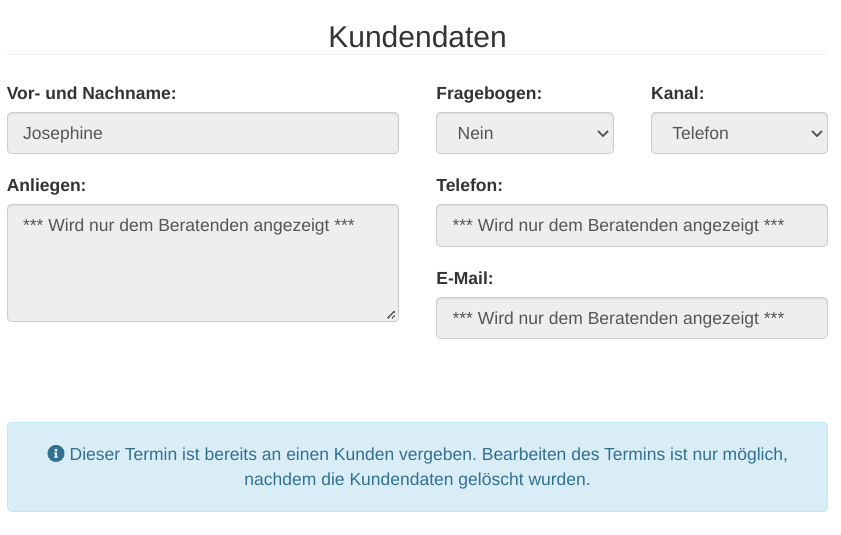
\includegraphics[width=0.9\textwidth]{screen_feedback_client_censorship.png}
\end{figure}


\begin{figure}[H]
    \caption{Neuer Button: Mit \textit{Speichern und Nächster} kann direkt der nächste Termin eingetragen werden.}
    \centering
    
\includegraphics[width=0.9\textwidth]{screen_feedback_save_next.png}
\end{figure}


\subsection{Reflektion der eingesetzen Methoden}

\paragraph{Human Centered Design und IIK}
% Einfache Umsetzung vs Nutzerfreundliche Lösung
% IIK sehr ertragreich, Prototypen wichtig für Feedback, Vorstellung

\paragraph{Implementierung und Usertests}
% Problem: Designpattern bei fertigem Softwareökosystem sehr eingeschränkt
% Fullcalendar Lib: Weniger Arbeit (billiger, robuster) dafür weniger Flexibilität
% Objektorientierter Ansatz sinnvoll für start serverlastige Anwendung?
% Evtl frühere Tests

\subsection{Zusammenfassender Abschluss}
% Eingehen auf Fragestellung der Einleitung
    % An welchen Stellen können die theoretischen Grundlagen des Human Centered Design den Entwicklungsprozess in der Praxis tatsächlich sinnvoll unterstützen? 
    % Gab es eventuell auch Methoden, die in der praktischen Umsetzung problematisch waren oder noch optimiert werden könnten?
    % Erfüllt die Software die gewünschten Anforderungen?
% Abrundendes Schlusswort

\subsection{Ausblick}
% Einführung neue Softwareversion (viel testen und abstimmen)
% Andere Module Überarbeiten
% Gruppentermine / Self Service einbuchen (Sicherheit)

%Literaturverzeichnis
\newpage
\bibliographystyle{apalike}
\bibliography{refs}

%Ende
\end{document}